\documentclass[12pt]{article}
\usepackage{graphicx,amssymb,amsmath,setspace,comment,verbatim,titling,pgf,lscape,color}
\usepackage[left=2cm,right=2cm,top=2.5cm,bottom=2cm]{geometry}
\usepackage[round]{natbib}
\usepackage{hyperref}
\usepackage{array}
\usepackage{bbm}
\usepackage{marginnote}
\usepackage[justification=centering]{caption}
%%\usepackage{breqn}
\usepackage{booktabs}
\newcommand{\pderiv}[2]{\frac{\partial#1}{\partial#2}}
%\usepackage{siunitx}
\newcolumntype{P}[1]{>{\raggedright\arraybackslash}p{#1}}
\hypersetup{colorlinks,%
						citecolor=black,%
						filecolor=black,%
						linkcolor=black,%
						urlcolor=blue,%
						}
\setstretch{1.5}

\setlength{\droptitle}{-50pt}

\begin{document}
\title{Decision Assistance and Steering in Health Insurance}
\author{Ian McCarthy \& Evan Saltzman}
\date{June 2021}
\maketitle

\vspace{-2ex}
\begin{abstract}
\noindent In many markets, consumers have access to an agent or some other intermediary to aid in decision making. The influence of such agents on consumer decisions, and the firm's influence on the behaviors of its agents, have important implications for the efficiency of these markets. In this paper, we study the welfare effects of decision assistance and firm steering in health insurance using the population of enrollments from the California Affordable Care Act (ACA) exchange from 2014 to 2019. We find that enrollees are nearly 2x more likely to select a silver plan when using some form of decision assistance and 30\% less likely to select a ``dominated'' plan. Preliminary results suggest that firms have considerable ability to steer consumers' decisions using agent commissions, where a \$1 increase in commissions paid to agents has the same effect as a \$2 or \$3 increase in plan premiums.
\end{abstract}

\clearpage

\section{Introduction}
\label{sec:introduction}

Health insurance markets are unique in many respects, not least of which is the increasing complexity of choosing an optimal health insurance plan. Such complexity has been well-documented in studies of health insurance choice in the Medicare Advantage market \citep{abaluck2011, ketcham2012, gruber2017}. One way to reduce the burden of this complexity is to provide professional decision support through private insurance agents or public assistance programs, both of which are available in the California health insurance exchanges created under the Affordable Care Act (ACA). Such decision assistance, however, also introduces the potential for private insurers to steer enrollees into potentially suboptimal plans. Commissions paid to facilitate any steering may also increase plan premiums for all enrollees. In this paper, we examine the role of decision assistance on health insurance plan choice and its implications for consumer welfare.

Our analysis is based on household enrollment data from the California ACA exchange. Our final data consist of over 3.2 million household-year observations from 2014 to 2019. The data include a variety of household characteristics, plan choices and plan characteristics, and information on the type of decision assistance used by the enrollee (if any). Using these data, we can precisely identify each household's choice set, the premium paid for each plan in the choice set, and any premium and cost sharing subsidies for which the household is eligible.

Our empirical analysis proceeds as follows. First, we examine whether decision assistance affects plan choice. Our estimand of interest is the average treatment effect on the treated (ATT) for enrollees receiving decision assistance. We employ as our estimator an augmented inverse propensity weighted nested logit regression, as discussed in more detail in Section \ref{sec:causal}, and we limit the analysis to newly enrolled households. We estimate that such households are 50\% more likely to select a silver plan and 20\% less likely to remain uninsured when using some form of decision assistance. We also find strong evidence of heterogeneous effects depending on the type of assistance used, wherein households using public decision assistance ...

Second, we consider the potential for decision assistance to ``improve'' plan choice. While identifying ``improvement'' is not generally feasible in our data, we can identify specific instances in which the observed plan choice is dominated by some other plan in an individual's choice set. For example, gold and platinum tier plans are dominated for any household that is eligible for cost-sharing subsidies and with incomes below 150\% of the federal poverty level. We can therefore identify dominated choices and examine whether those with decision assistance appear less likely to select a dominated plan. As with our initial nested logit model of plan choice, our estimand is the ATT for households receiving decision assistance, and our estimator is an augmented inverse propensity weighted logit regression. 

Regarding dominated choices, our results suggest that individuals with decision assistance are over 1 percentage point less likely to make a dominated choice. On a base of 3.5\%, this reflects a 30\% decrease in the probability of making a dominated choice. We again find evidence of heterogeneities in the effects of different forms of decision assistance. In particular, we find that individuals using publicly provided decision assistance are around 0.8 percentage points less likely to select a dominated plan, while individuals using a private insurance agent are 1.2 percentage points less likely to select a dominated plan.

Third, 

We contribute to two distinct literatures. First, our examination of decision assistance and health insurance relates to the literature on the role of experts in decision making.

A related literature considers the effects of recommendations, sometimes automated via an algorithmic recommendation, on decisions. \cite{bundorf2019}, for example, show that offering additional information alongside an algorithmic expert recommendation significantly affects an individual's choice of prescription drug plans.

Second, we contribute to the literature examining the prevalence and underlying mechanisms of poor decision making in health insurance. In the employer-provided insurance market, \cite{liu2021} documents that over half of employers offer a dominated plan among their menu of insurance options available to their employees, and \cite{sinaiko2011} and \cite{bhargava2017} find that a large share of employees regularly select such dominated insurance plans. \cite{abaluck2011}, \cite{ketcham2012}, \cite{zhou2012}, \cite{heiss2013}, \cite{gruber2017}, \cite{ho2017rand} and many others similarly examine poor decisions when selecting a Medicare prescription drug (Part D) plan. The consensus from this literature is that individuals regularly make \textit{ex ante} very bad health insurance decisions, often selecting plans that are either financially dominated by other plan options or most likely suboptimal given the enrollee's existing medical conditions.

Specifically in the context of the ACA, \cite{orzol2018} find that an ``Enroll America,'' a national non-profit organization designed to expand health insurance enrollment in the U.S., significantly increased enrollment in the ACA exchange plans. \cite{myerson2019} also finds that federally funded assistance programs significantly increased the probability of enrollment in Medicaid, although they found little effect of such federal funding on enrollment in exchange plans. \cite{sommers2015} similarly show that access to navigators is highly correlated with Medicaid enrollment, mirroring earlier findings from \cite{aizer2003} in her study of Medicaid enrollment and application assistants in California.

\cite{aizawa2021}

While not definitive, a common theme in this literature is that poor health insurance decisions are due in-part to an inability or unwillingness of enrollees to accurately evaluate their plan options \citep{bhargava2017, hanoch2009}. Even still, \cite{ketcham2012} find that any such poor decision making will tend to improve over time, thereby partially alleviating the need for any explicit intervention. 


\section{Background and Institutional Details}
\label{sec:background}

One of the pillars of the Affordable Care Act (ACA) was the creation of regulated state insurance exchanges in which insurers sell private insurance plans directly to consumers. Although all state exchanges must adhere to a minimum set of regulations, there exists significant variation across states in terms of how they manage and regulate their exchanges. Since our analysis uses data from the California exchange, we focus our discussion on California.

There are three general aspects of the California insurance exchange that are particularly relevant for our analysis: 1) enrollee choice sets and the types of plans available; 2) variation in premiums across individuals on the exchange; and 3) the presence of navigators and brokers to assist individuals when considering an exchange plan. We discuss the institutional details of each of these areas in more detail throughout the remainder of this section.

\subsection{Choice Sets and Plan Types}
Exchange plans are classified by a ``metal'' tier intended to easily summarize the actuarial value (AV) of a plan. Bronze plans reflect an AV of 60\%, silver plans an AV of 70\%, gold plans an AV of 80\%, and platinum plans an AV of 90\%. For plans on the California exchange, other cost sharing parameters are standardized within a metal tier, such that the enrollee's financial burden across plans within a given metal tier is relatively homogeneous.\footnote{In other states, insurers can generally design plans with different cost sharing provisions within a metal tier, but the regulations on the California exchange are more stringent.} Each state also defines geographic rating areas, usually composed of counties, in which an insurer's premiums must be the same for consumers of the same age.

Most households face the same choice set based on their region and year of enrollment; however, some individuals (mainly those under age 30) are also eligible for basic catastrophic coverage. Insurers can also choose to serve only a part of a rating area. Such ``partial'' rating area coverage is relatively uncommon in California, and \cite{fang2020} show that insurers' decisions to enter a subset of counties in a rating area appears to be determined by entry costs and risk pools rather than strategic competitive behavior.

\subsection{Premiums and Cost-sharing}
Premium variation within a plan is more tightly regulated in California than in other state exchanges, with insurer price discrimination only allowed based on an enrollee's age and geographic residence. For example, insurers can charge a 64-year old up to 3 times as much as a 21-year old according to the default age rating curve.

The ACA also provides premium and cost-sharing subsidies to eligible enrollees.\footnote{Premium subsidies are available to consumers who meet the following criteria: 1) income between 100 and 400\% of the federal poverty level (FPL); 2) citizenship or legal resident status; 3) ineligible for public insurance such as Medicare or Medicaid; and 4) lack access to an ``affordable plan offer'' through employer-sponsored insurance either as an employee or as a dependent. Cost-sharing subsidies are available to anyone with income $\leq$ 250\% of FPL and serve to increase the actuarial value of a plan from 70\% up to 94\% (income $<$ 150\% of FPL), 87\% (income between 150\% and 200\% of FPL), and 73\% (incomes between 200\% and 250\% of FPL).} The premium subsidy is set to the difference between: 1) the premium of the benchmark plan, defined as the second-cheapest silver plan available to a given enrollee; and 2) and the enrollee's income contribution cap, defined as the maximum percent of a person's income spent on premiums. Consumers can apply the premium subsidy towards the premium of any metal plan, whereas cost-sharing subsidies only apply to the purchase of a silver tier plan.

\subsection{Decision Assistance}
There are two forms of formal decision assistance available to potential enrollees on the California exchange: publicly funded ``navigators'' and private insurance agents or brokers. For states participating in the federal exchange, navigators are mandated under the ACA and federally funded. Navigators are voluntary for state-based exchanges, although most states offer such assistance to potential enrollees, including California. 

A navigator is essentially a public employee available to help potential enrollees better understand their insurance options. Access to navigators has been shown to have a particularly large effect on Medicaid enrollment \citep{myerson2019, sommers2015, aizer2003}. Relatedly, navigators tend to work with households of lower incomes, currently uninsured, and non-native english speakers. Among individuals receiving some form of assistance in our data, about 30\% of households used a navigator.

Potential enrollees on the California exchange may also use a traditional private insurance agent or broker (hereafter, agents). Agents are not generally tied to any specific insurer and can enroll individuals in any available plans. Agents are also not restricted to any specific geography or region and can enroll individuals in the relevant rating area regardless of the physical office in which the agent resides. Among individusl receiving some form of assistance in our data, 70\% used a private insurance agent.

Unlike navigators, agents are paid commissions for each enrollment into an exchange plan. The amount of commission varies by insurer and is generally set as a flat fee per enrollee or as a percentage of the premium paid by that enrollee. For new enrollees, flat fee commissions typically range between \$100 and \$200, with percent commissions ranging between 2\% and 5\%. Figure~\ref{fig:commissions} presents the observed commission rates by insurer over time, separately among insurers offering a flat fee commission versus those offering a percentage commission. As is evident from the figure, there exists relatively large variation in commissions across insurers, as well as within-variation over time for large insurers such as Anthem, Health Net, and Blue Shield.


\section{Data}
\label{sec:data}
We have detailed individual and household-level administrative data from California's ACA exchange (i.e., Covered California) from 2014-2019. The data indicate each enrollee's selected plan and key demographic information, including age, income, county of residence, subsidy eligibility, and household composition. We also collect data on plan characteristics and rate filings, including the plan premium, metal tier, cost sharing requirements (e.g., deductible, coinsurance, and maximum out-of-pocket limit), and network type (e.g., HMO, PPO). Demographic and plan characteristics allow the construction of each household's menu of plan choices and household-specific premiums, $p_{ij}$. Individual and household identifiers allow consumers to be grouped into household units and tracked across time.\footnote{To form the universe of \textit{potential} exchange consumers, we supplement the Covered California data with data from the American Community Survey (ACS). From the full ACS data, we exclude individuals enrolled in or eligible for another source of insurance coverage as well as those ineligible to purchase insurance on the exchanges. Details of ACS data are described in the supplemental appendix.} 

Our final data consist of 8.3 million total households from 2014-2019. Of these, 4.5 million were not previously enrolled in any Covered California plan in the prior year. Table~\ref{tab:summary-stats} displays summary statistics for all households in our data. Since the key independent variable throughout much of our analysis is whether a household used some form of decision assistance, we present summary statistics separately between those that used and did not use decision assistance. 

We see from Table~\ref{tab:summary-stats} that enrollees using decision assistance are of lower income and larger household size. Among types of plans purchased, we see little difference between those with and without decision assistance, with the exception of Kaiser plans for which individuals using decision assistance are less likely to purchase. Overall, the silver tier is the most commonly selected option, and this is particularly true for those using decision assistance. Enrollees with decision assistance are also much more likely to select an HMO and relatively more likely to select a PPO.


\section{Decision Assistance and Plan Choice}
\label{sec:causal}

\subsection{Estimation}
\label{subsec:causal-methods}
We model health insurance purchasing with a nested logit discrete choice model, as in \cite{saltzman2019}, and we derive estimates of the effect of decision assistance by embedding this discrete choice model into a potential outcomes framework \citep{rubin1974, imbens2009}.

For our nested logit discrete choice model, we assume that household $i$ chooses the plan $j$ that maximizes their utility,
\begin{equation}
u_{ij} = \alpha_{i}p_{ij} + \beta x_{j} + \gamma d_{i} + \xi_{j} + \varepsilon_{ij}, 
\label{eqn:utility}
\end{equation}
where $p_{ij}$ denotes the premium for plan $j$, $x_{j}$ denotes a vector of product characteristics, $d_{i}$ denotes a vector of household characteristics, $\xi_{j}$ captures unobserved product characteristics, and $\varepsilon_{ij}$ is an error term assumed to follow a type I extreme value distribution. We allow for heterogenities in price elasticities across households by parameterizing $\alpha_{i}$ in Equation~\eqref{eqn:utility}, $\alpha_{i} = \alpha + \theta d_{i}.$ In our estimation, this amounts to including interactions between $d_{i}$ and $p_{ij}$.

Using the nested logit model in Equation~\eqref{eqn:utility}, our goal is to estimate the average treatment effect on the treated (ATT), which in our case reflects the average treatment effect among those using some form of decision assistance. To allow for general heterogeneous treatment effects, we estimate the ATT with a four-step process: 
\begin{enumerate}
    \item Estimate the nested logit model of plan choice from Equation~\eqref{eqn:utility}, limiting the sample to those observed to \textbf{not} have used any form of decision assistance. We estimate Equation~\eqref{eqn:utility} separately for each year and region, implicitly allowing for a full set of region/year interactions among all covariates. For this reason, we select a relatively small set of covariates, including household-specific premiums, the interaction between premiums and household size, the actuarial value of the plan, the metal tier, indicators for network type (HMO or PPO), and insurer fixed effects. We then obtain a set of coefficient estimates, $\hat{\theta} = \{\hat{\alpha}, \hat{\beta}, \hat{\gamma}, \hat{\xi} \}$.\footnote{These coefficient estimates differ by region and year, but we supress that notation for brevity.}

    \item Use $\hat{\theta}$ to form the predicted counterfactual, $\widehat{Pr[Y_{ij}^{0} | \text{Assistance}]}$. In other words, we use the results of our choice model, estimated only among those without decision assistance, to predict the counterfactual outcome of plan choice among those that \textbf{did} use some form of decision assistance.

    \item Sum the predicted probabilities across individuals, $$\widehat{N_{j}^{0}} = \sum_{ i \in \Omega} \widehat{Pr[Y_{ij}^{0} | \text{Assistance}]},$$ where $\Omega$ denotes the set of all enrollees that used decision assistance. Among such enrollees, this reflects the predicted number of enrollments if enrollees had not used any assistance.
    
    \item Sum the observed number of enrollments, $N_{j}^{1}$, and take the difference between this and the counterfactual prediction,
    \begin{equation}
        ATT_{j} = \underbrace{N^{1}_{j}}_{Observed} - \underbrace{\widehat{N_{j}^{0}}}_{Predicted}.
    \label{eqn:att}
    \end{equation}
\end{enumerate}

Interpreting Equation~\eqref{eqn:att} as an estimate of the ATT assumes that individuals receiving decision assistance do not seek assistance due to some unobserved factors that also affect their plan choice. Conditional on household characteristics as well as insurer fixed effects, (implicitly) interacted with a full set of region and year fixed effects, we argue that this assumption is plausible; however, our estimation strategy employs untreated households (i.e., those without decision assistance) to predict counterfactual choices for treated households and therefore requires sufficient balance between treated and untreated households. As is evident from Table~\ref{tab:summary-stats}, there is reason to suspect that such balance does not hold in our data.

To ensure balance among observed covariates, we employ an augmented inverse propensity weighted regression estimate \cite{wooldridge2010}, in which the weights in the nested logit estimation derive from a preliminary logit regression of decision assistance status for each household. The outcome in this preliminary regression is an indicator variable, set to one if a household used decision assistance (i.e., the treatment group) and 0 otherwise (i.e., the control group). Denoting the resulting predicted probability of decision assistance by $\hat{p}_{i}$, we then assign a weight of $\frac{\hat{p}_{i}}{1-\hat{p}_{i}}$ to each observation in the control group and proceed with step (1) above using these weights in the nested logit regression. Conceptually, this approach assigns more weight to households without decision assistance that are ``most similar'' to households that use decision assistance.


\subsection{Results}
\label{subsec:causal-results}

Figure~\ref{fig:ps-balance} presents the resulting propensity scores from our preliminary logit regression of decision assistance against observable household demographics. As is evident from the figure, there exists common support in propensity scores for the treated and control groups. In Figure~\ref{fig:cov-balance}, we present a comparison of observable household characteristics between the treatment and control groups. The hollow circles in Figure~\ref{fig:cov-balance} reflect the unadjusted differences in means, while the solid circles reflect the difference in means when weighting households. Weights for treated households are set to 1, and weights for untreated households are set to  $\frac{\hat{p}_{i}}{1-\hat{p}_{i}}$ based on the preliminary logistic regression. We see from Figure~\ref{fig:cov-balance} that our treated and control groups are well-balanced after weighting.

We summarize our ATT estimates by insurer and metal tier, presented in Figures~\ref{fig:choice-insurer} and \ref{fig:choice-metal} respectively. Figure~\ref{fig:choice-insurer} shows that individuals using decision assistance are significantly more likely to select a plan offered by Blue Shield, Health Net, or another smaller insurer, and much less likely to select a plan offered by Anthem or Kaiser. Of note, Anthem and Kaiser are similar in that they both offer flat commission payments. Kaiser sets the lowest of all such flat commissions in all years, while Anthem dropped their commission payments dramatically beginning in 2015. We investigate the issue of commission and plan choice more fully in Section \ref{sec:steering}.

With regard to metal tier, Figure~\ref{fig:choice-metal} shows that individuals with decision assistance are about 16 percentage points more likely to select a silver tier plan. With xx\% of unassisted households selecting a silver plan, this reflects a relative increase of xx\% in the probability of selecting a silver plan. Most of this increase comes from a reduction in the probability of selecting a bronze plan, with a smaller (but still significant) reduction in selecting gold plans.


\section{Dominated Choices}
\label{sec:dominated}
The results in Section~\ref{subsec:causal-results} reveal large effects of decision assistance on plan choice; however, it is not clear from those results whether decision assistance \textit{improves} plan choice or simply reallocates households into different, perhaps worse, plans. 

To examine this question, we first identify specific instances in which the observed plan choice is dominated by some other plan in an individual's choice set, and we estimate the effects of decision assistance on the probability of making such a choice. For example, for any household that is eligible for cost-sharing subsidies and with incomes below 150\% of the federal poverty level (FPL), silver plans will have lower premiums and lower out-of-pocket costs compared to gold or platinum tier plans such that the actuarial value of silver plans exceeds that of gold and platinum plans. Since provider networks are not allowed to vary across metal tiers for the same plan type, gold and platinum plans are strictly dominated by silver plans for such households. Gold plans are similarly dominated by silver plans for households with incomes between 150\% and 200\% of the FPL. 

We estimate the effect of decision assistance on dominated choices with a logistic regression, in which the outcome is an indicator for whether the enrollee made a dominated choice. Individuals that do not have a dominated plan in their choice set are excluded. Following the process laid out in Section~\ref{sec:causal}, we estimate a weighted logistic regression model only among individuals without any decision assistance, with weights derived from a preliminary logit regression of decision assistance against observable household characteristics. We then use the coefficient estimates to form predicted counterfactual probabilities for dominated choices among individuals that did use decision assistance. Finally, again limiting to those with decision assistance, our estimate of the ATT is the average probability of a dominated choice less the average predicted probability of a dominated choice.

Results are presented in Figure~\ref{fig:dom-choice}, where we show the point estimate and 95\% confidence interval for the ATT. We also report the mean proportion of dominated choices observed in the data. We present different ATTs for people with any decision assistance and for those specifically using public navigators versus private insurance agents. We estimate that individuals are just over 1 percentage point less likely to make a dominated choice when using any form of decision assistance. On a base of 3.5\%, this reflects a nearly 30\% reduction in the prevalence of dominated choices. These effects are largest among those using a private insurance agent, where we estimate an ATT of -1.2 percentage points compared to an ATT of -0.8 percentage points for individuals using a navigator.


\section{Welfare and Insurer Steering}
\label{sec:steering}

\subsection{Model}
\label{subsec:steering-model}

Consider a two-stage  game where  (1) firms set premiums and commissions simultaneously to maximize their expected profit and (2) consumers select a plan to maximize their expected utility. In the following three subsections, we detail how we (1) model the decisions of firms; (2) model the decisions of consumers; and (3) find the model equilibrium.  

Given our available data, we do not explicitly model the actions of individual insurance agents.  However, we do model how firms use agent compensation to steer an agent's clients to their plans.  Our approach assumes that the consumer's decision to seek agent assistance is independent of the firms' commission levels.  This identifying assumption is valid if commissions incentivize agents to recommend certain plans to their clients, but do not induce agents to change advertising levels or marketing efforts to  seek new clients. Advertising and marketing by both insurers and agents are tightly regulated, particularly in Covered California.  We therefore believe our identifying assumption is relatively  innocuous.   

\subsubsection{Stage 1: Firms Set Premiums and Commissions}

\paragraph{Firm Decision Variables:}
Firms set premiums and commissions to maximize their expected profit.  Let $p_{jmt}$ be the base premium decision for each plan $j$ sold in market $m$ in period $t$ and the \textit{commission decision} $n_{gjt}$ 

\vspace{-0.4in}		
\singlespacing
\begin{eqnarray*}
    n_{gjt}  \equiv 
    \begin{cases} 
	    \delta_{gjt} & \mathrm{\% \,\, commission} \\		
	    \eta_{gjt} & \mathrm{\$ \,\, commission} \\
	    0 & \mathrm{o/w}
    \end{cases}
\end{eqnarray*}		   
\doublespacing
\noindent for each plan $j$ sold at time $t$ with renewal status $g$ (i.e., new or existing customer). Agents are either paid a percentage $\delta_{gjt}$  of the consumer's unsubsidized premium  or a flat amount $\eta_{gjt}$ that is independent of the premium.  We assume the firm's decision to pay a percentage commission or flat commission is exogenous because switching agent compensation methods is costly.  The only firm that switched between compensation methods during our six-year study timeframe was Health Net following its acquisition by Centene. The \textit{commission paid} to household $i$'s insurance agent is

\vspace{-0.4in}		
\singlespacing			
\begin{eqnarray*}
	\eta_{gijt}(\textit{p},\textit{n})  \equiv 
	\begin{cases} 
		n_{gjt} \left(\sigma_{it}p_{jmt}\right) & \mathrm{\% \,\, commission} \\		
		n_{gjt} & \mathrm{\$ \,\, commission}
    \end{cases},
\end{eqnarray*}
\doublespacing
\noindent where $\textit{p} = {\bf p}_t$ is the vector of plan base premiums set by all insurers in each market in year $t$, $\textit{n} = {\bf n}_t$ is the vector of commission decision variables in period $t$, and the household's (unsubsidized) premium is the product of the household's rating factor $\sigma_{it}$  and the plan's base premium $p_{jmt}$. In California, the rating factor can vary by age and geographic residence of the household's members.\footnote{The ACA also permits rating by tobacco usage, but California prohibits tobacco rating.}  Insurers can charge a 64-year-old up to 3 times as much as a 21-year-old. Figure~\ref{rating_area_partitions} shows the partition of California into rating areas.  In each rating area,  an insurer's premium must be the same for all consumers of the same age. Total commissions paid by firm $f$  are		
	
\vspace{-0.2in}		
\begin{equation*}
    \mathcal{C}_{ft}(\textit{p},\textit{n};\boldsymbol{\theta}) = \sum_{g \in G, i \in I, m\in M, k \in J_{fmt}} \left( \mathbb{I}_{n,i,t} \right)  q_{ikt}(\textit{p},\textit{n};\boldsymbol{\beta}) \eta_{gikt}(\textit{p},\textit{n}),
\end{equation*}
where $\mathbb{I}_{n,i,t}$ indicates whether household $i$ is assisted by an agent in year $t$, $q_{ikt}(\cdot)$ is the probability household $i$ chooses plan $k$ at time $t$, and $J_{fmt}$ is the set of plans offered by firm $f$ in market $m$ at time $t$.  The model parameters $\boldsymbol{\theta} \equiv (\boldsymbol{\beta},\boldsymbol{\gamma},\boldsymbol{\mu})$, where $\boldsymbol{\beta}$ are the demand parameters, $\boldsymbol{\gamma}$ are the risk score parameters, and $\boldsymbol{\mu}$ are the average claims parameters.


\paragraph{Risk Adjustment Transfers:} 
\citet{Pope2014} derive the ACA risk adjustment transfer formula.\footnote{We start with \citet{Pope2014}'s transfer formula as derived in their first appendix, which allows plans to vary only by their actuarial values (and not by differences in firm efficiency, geographic costs, allowable rating factors, or moral hazard).  We start with this formula because we want to capture all differences in expected risk, except for cost sharing and any associated moral hazard, in the plan's risk score (i.e., cost sharing and moral hazard are addressed through the utilization share).  In contrast, the plan liability risk score   $PLRS_j$ as defined in \citet{Pope2014}'s second appendix does not account for certain differences such as variation in geographic cost.  Instead, \citet{Pope2014} account for these differences by applying factors in the transfer formula.}  In our notation, the per-member per-month risk adjustment transfer $ra_{jmt}(\textit{p},\textit{n};\boldsymbol{\theta})$ for plan $j$ is

\vspace{-0.2in}
\begin{equation*}
	ra_{jmt}(\textit{p},\textit{n};\boldsymbol{\theta}) = \left(\frac{r_{jmt}(\textit{p},\textit{n};\boldsymbol{\theta})\sum_{m \in M, l \in J_{mt}} q_{lmt}(\textit{p},\textit{n};\boldsymbol{\beta})}{\sum_{m \in M, l \in J_{mt}} r_{jmt}(\textit{p},\textit{n};\boldsymbol{\theta}) q_{lmt}(\textit{p},\textit{n};\boldsymbol{\beta})}    -     \frac{h_j\sum_{m \in M, l \in J_{mt}} q_{lmt}(\textit{p},\textit{n};\boldsymbol{\beta})}{\sum_{m \in M, l \in J_{mt}} h_l q_{lmt}(\textit{p},\textit{n};\boldsymbol{\beta})}\right)\overline{p},
\end{equation*}
where $r_{jmt}(\cdot)$ is the plan risk score, $h_j$ is an exogenous expected utilization factor set by regulation that accounts for the plan AV and any associated moral hazard, and $\overline{p}$ is the weighted average premium in the market.  The plan's total risk adjustment transfer $RA_{jmt}(\textit{p},\textit{n};\boldsymbol{\theta})$ equals

\vspace{-0.4in}
\begin{eqnarray}
\label{eqn:ra_formula}
	RA_{jmt}(\textit{p},\textit{n};\boldsymbol{\theta}) &=& ra_{jmt}(\textit{p},\textit{n};\boldsymbol{\theta})  q_{jmt}(\textit{p},\textit{n};\boldsymbol{\beta}) \nonumber \\
	&= & \left[rs_{jmt}(\textit{p},\textit{n};\boldsymbol{\theta})  - us_{jmt}(\textit{p},\textit{n};\boldsymbol{\theta})  \right] R_t(\textit{p},\textit{n};\boldsymbol{\beta}),
\end{eqnarray}
where $rs_{jmt}(\cdot)$ is the plan's ``risk share'' of total claims, $us_{jmt}(\cdot)$ is the plan's ``utilization share'' of total claims, and $R_t(\cdot) = \sum_f R_{ft}(\cdot)$ is total premium revenue across all plans. The total risk adjustment transfer for the firm equals the sum of the risk adjustment transfers for the plans that it sells (i.e., $RA_{ft}(\cdot) = \sum_{m \in M, j \in J_{fmt}} RA_{jmt}(\cdot)$.
	
The plan's risk share includes the combined effects of adverse selection, moral hazard, and plan AV, whereas the plan's utilization share only includes the effects of moral hazard and plan AV. Thus, the difference between the risk share and utilization share captures the plan's relative risk due to adverse selection only. The risk share equals

\vspace{-0.1in}
\begin{equation*}
	rs_{jmt}(\textit{p},\textit{n};\boldsymbol{\theta}) = \frac{ r_{jmt}(\textit{p},\textit{n};\boldsymbol{\theta}) q_{jmt}(\textit{p},\textit{n};\boldsymbol{\beta})}{\sum_{m \in M, l \in J_{mt}}  r_{lmt}(\textit{p},\textit{n};\boldsymbol{\theta}) q_{lmt}(\textit{p},\textit{n};\boldsymbol{\beta})},
\end{equation*}
where $J_{mt}$ is the set of all plans offered in market $m$ and year $t$, and the plan risk score $r_{jmt}(\cdot)$ is a function of enrollee characteristics and the plan AV. We do not directly observe plan risk scores in the insurer rate filing data.  However, we observe all other variables in Equation~\eqref{eqn:ra_formula}, including each plan's risk adjustment transfer, and can therefore solve for the plan risk scores. The plan's utilization share $us_{jmt}(\cdot)$ equals

\vspace{-0.1in}
\begin{equation*}
	us_{jmt}(\textit{p},\textit{n};\boldsymbol{\theta}) =  \frac{ h_j q_{jmt}(\textit{p},\textit{n};\boldsymbol{\beta})}{\sum_{m \in M, l \in J_{mt}} h_l q_{lmt}(\textit{p},\textit{n};\boldsymbol{\beta})}.
\end{equation*}
A positive difference between the risk share and the utilization share indicates that a plan has high risk relative to its expected utilization and results in the plan receiving a risk adjustment transfer; a negative difference indicates that a plan has low risk relative to its expected utilization and results in the plan paying a risk adjustment transfer.

\paragraph{Calculating Variable Profit:} 
Firms choose premiums and commissions to maximize expected variable profit

\vspace{-0.4in}		
\begin{footnotesize}
\begin{eqnarray}
\label{eqn:profit}
	\pi_{ft}(\textit{p},\textit{n};\boldsymbol{\theta}) &=&  R_{ft}(\textit{p},\textit{n};\boldsymbol{\theta}) -  C_{ft}(\textit{p},\textit{n};\boldsymbol{\theta}) - \mathcal{C}_{ft}(\textit{p},\textit{n};\boldsymbol{\theta}) + RA_{ft}(\textit{p},\textit{n};\boldsymbol{\theta}) +  RI_{ft}(\textit{p},\textit{n};\boldsymbol{\theta})  - V_{ft}(\textit{p},\textit{n};\boldsymbol{\theta})  \nonumber \\
	&=& R_{ft}(\textit{p},\textit{n};\boldsymbol{\theta}) - (1 - \iota_{ft}) C_{ft}(\textit{p},\textit{n};\boldsymbol{\theta}) - \mathcal{C}_{ft}(\textit{p},\textit{n};\boldsymbol{\theta}) + RA_{ft}(\textit{p},\textit{n};\boldsymbol{\theta})   - V_{ft}(\textit{p},\textit{n};\boldsymbol{\theta}),
\end{eqnarray}
\end{footnotesize}

\noindent where $R_{ft}(\cdot)$ is total premium revenue, $C_{ft}(\cdot)$ is total claims, $RI_{ft}(\cdot)$ is reinsurance received, $V_{ft}(\cdot)$  is variable administrative cost (excluding commissions), and $\iota_{ft}$ is the actuarial value of the reinsurance contract (i.e., the expected percentage of claims paid by the reinsurer).  Total commissions paid $\mathcal{C}_{ft}(\cdot)$ and risk adjustment received  $RA_{ft}(\cdot)$ are as above.


\subsubsection{Stage 2: Household Plan Choice}
Households choose the plan that maximizes their (indirect) utility function

\vspace{-0.4in}
\begin{eqnarray}
\label{eqn:demand_model}
	U_{ijt}(\textit{p},\textit{n};\boldsymbol{\beta}) &\equiv& \beta_{i}^p p_{ijt}(\textit{p}) + \beta_j^{\eta} \eta_{gijt}(\textit{p},\textit{n})   + \beta_i^y y_{ij(t-1)} + x'_{ij}\beta^x + \xi_{j} + \epsilon_{ijt}^d, 
\end{eqnarray}
where $p_{ijt}(\textit{p})$ is household $i$'s (subsidized) premium for plan $j$ in year $t$, $\eta_{gijt}(\textit{p},\textit{n})$ is the commission paid to household $i$'s insurance agent, $y_{ij(t-1)}$ indicates whether household $i$ chose plan $j$ in the previous year, $x_{ij}$ is a vector of observed product characteristics including the plan AV,  $\xi_{j}$ is a vector of unobserved product characteristics, and $\epsilon_{ijt}^d$ is an error term.  CSRs enter utility through the plan AV and premium subsidies reduce the household's premium $p_{ijt}(\textit{p})$.   The utility of the outside option $U_{i0t} = \beta_i^p \rho_{it} + \epsilon_{i0t}$, where $\rho_{it}$ is the household's penalty for not having insurance in year $t$. 

The household's premium is calculated as

\vspace{-0.4in}
\begin{eqnarray}
\label{eqn:cons_premium}
	p_{ijt}(\textit{p}) &=& \max \left \lbrace \underbrace{\sigma_{it} p_{jmt}}_{\text{\scriptsize{full premium}}}  - \underbrace{\max\{\sigma_{it} p_{bmt} - \zeta_{it},0\}}_{\text{\scriptsize{premium subsidy}}},0 \right \rbrace, 
\end{eqnarray}
where $\sigma_{it}$ is the household's rating factor as before, $p_{bmt}$ is the base premium of the benchmark plan in market $m$ and year $t$, and $\zeta_{it}$ is the household's income contribution cap.  The household's premium subsidy equals the difference between what the household would pay for the benchmark plan (i.e., $\sigma_{it} p_{bmt}$) and the household's income contribution cap $\zeta_{it}$. The benchmark plan is the second-cheapest silver plan available to the household and varies between consumers because of heterogeneous firm entry. The income contribution cap ranged from $2\%$ of annual income for consumers earning $100\%$ of the federal poverty level (FPL) and $9.5\%$ of annual income for consumers earning $400\%$ of FPL in 2014. The income contribution caps increase slightly each year. Subsidies can be applied to any plan except a catastrophic plan. For some low-income consumers, the premium subsidy may exceed the full premium of certain bronze plans. The subsidy is reduced in these cases to ensure nonnegativity of the premium. 

We define the vector of demand parameters $\boldsymbol{\beta} \equiv (\beta_i^p,\beta_j^{\eta},\beta_i^y,\beta^x)$ to accommodate heterogeneous consumer preferences.  The household's premium parameter $\beta_{i}^p \equiv \beta^p + w'_{it} \phi$ varies with household characteristics $w_{it}$.  The household's inertia parameter $\beta_i^y = \beta^y +  x'_{ij} \kappa + w'_{it} \nu$ varies with both household and product characteristics. The steering parameter $\beta_j^{\eta}$ captures the degree to which agent compensation steers  an agent's clients to particular plans.  A high value of $\beta_j^{\eta}$ would indicate that agent compensation is effective in steering consumers.   Because smaller firms offer agents considerably higher commissions, we allow the steering parameter to vary with firm size.


\paragraph{Calculating Demand}
We assume Equation~\eqref{eqn:demand_model}) is a nested logit model such that the vector of error terms $\epsilon_i$ has the generalized extreme value distribution.  The first nest contains all exchange plans and the second nest contains only the outside option.  This two-nest structure captures the key observed substitution pattern between the silver tier and the outside option resulting from the ACA's linkage of CSRs to the purchase of silver plans. Under the assumption that $\epsilon_i$ has the generalized extreme value distribution, the household choice probabilities are 

\vspace{-0.4in}		
\begin{eqnarray}
\label{eqn:choice_probs}
	q_{ijt}(\textit{p},\textit{n};\boldsymbol{\beta}) &=&  \frac{e^{V_{ijt}(\textit{p},\textit{n};\boldsymbol{\beta})/\lambda}\left(\sum_{j } e^{V_{ijt}(\textit{p},\textit{n};\boldsymbol{\beta})/\lambda}\right)^{\lambda-1}}{1 + \left(\sum_{j} e^{V_{ijt}(\textit{p},\textit{n};\boldsymbol{\beta})/\lambda}\right)^{\lambda}},
\end{eqnarray}
\noindent where $V_{ijt}(\textit{p},\textit{n};\boldsymbol{\beta}) \equiv \beta_{i}^p p_{ijt}(\textit{p}) + \beta_j^{\eta} \eta_{gijt}(\textit{p},\textit{n})   + \beta_i^y y_{ij(t-1)} + x'_{ij}\beta^x + \xi_{j}$ and $\lambda$ is the nesting parameter. The household choice probabilities in Equation~\eqref{eqn:choice_probs} converge to the standard logit choice probabilities when $\lambda \rightarrow 1$.

The sensitivity of a subsidized consumer's demand $q_{ijt}(\textit{p})$ to a premium change is given by  

\vspace{-0.4in}
\begin{eqnarray*}
	\frac{\partial q_{ijt}(\textit{p},\textit{n};\boldsymbol{\beta})}{\partial p_{jmt}} &=& \sum_{l \in J_{mt}} \frac{ \partial q_{ijt}(\textit{p},\textit{n};\boldsymbol{\beta})}{\partial p_{ilt}(\textit{p})}\frac{ \partial p_{ilt}(\textit{p})}{\partial p_{jmt}}
\end{eqnarray*}
\noindent for all plans $j,k$ in the set of available plans $J_{mt}$.  Assuming a strictly positive subsidy that does not exceed the full, unsubsidized premium, it follows from Equation~\eqref{eqn:cons_premium} that

\vspace{-0.4in}
\singlespacing
\begin{eqnarray}
\label{eqn:price_partial_formula}
    \frac{\partial p_{ilt}(\textit{p})}{\partial p_{jmt}} = 
    \begin{cases} 
	    0 & l=j, j = b \\		
		\sigma_{it} & l = j, j \neq b \\     
		-\sigma_{it} & l \neq j, j = b \\
		0 & l \neq j, j \neq b  
    \end{cases}.
\end{eqnarray}
\doublespacing
For a non-benchmark plan, an infinitesimal premium increase results in consumers paying more for that plan only.  An infinitesimal increase in the benchmark premium does not affect what subsidized consumers pay for the benchmark plan, but reduces what consumers pay for all other plans because of the larger subsidy. The complex relationship between insurer and consumer premiums, endogenous determination of the benchmark premium, and variation in the benchmark plan across consumers due to heterogeneous entry create significant computational challenges for estimation.  We carefully model the endogenous subsidy design despite the high computational cost because of the critical role premium subsidies play in addressing adverse selection.  

\subsubsection*{Equilibrium}

Now we find the first-order necessary conditions for a Nash equilibrium.  Differentiating Equation~\eqref{eqn:profit} with respect to the premium and the commission yields the  first-order conditions  

\vspace{-0.4in}	
\begin{footnotesize}
\begin{eqnarray}
\label{eqn:acara_foc_short}
	\frac{\partial R_{ft}(\textit{p},\textit{n};\boldsymbol{\theta})}{\partial p_{jmt}} + \frac{\partial RA_{ft}(\textit{p},\textit{n};\boldsymbol{\theta})}{\partial p_{jmt}} &=& (1-\iota_{ft}) \frac{\partial C_{ft}(\textit{p},\textit{n};\boldsymbol{\theta})}{\partial p_{jmt}} + \frac{\partial \mathcal{C}_{ft}(\textit{p},\textit{n};\boldsymbol{\theta})}{\partial p_{jmt}} + \frac{\partial V_{ft}(\textit{p},\textit{n};\boldsymbol{\theta})}{\partial p_{jmt}} \nonumber \\
	\frac{\partial R_{ft}(\textit{p},\textit{n};\boldsymbol{\theta})}{\partial n_{gjt}} + \frac{\partial RA_{ft}(\textit{p},\textit{n};\boldsymbol{\theta})}{\partial n_{gjt}} &=& (1-\iota_{ft}) \frac{\partial C_{ft}(\textit{p},\textit{n};\boldsymbol{\theta})}{\partial n_{gjt}} + \frac{\partial \mathcal{C}_{ft}(\textit{p},\textit{n};\boldsymbol{\theta})}{\partial n_{gjt}} + \frac{\partial V_{ft}(\textit{p},\textit{n};\boldsymbol{\theta})}{\partial n_{gjt}}
\end{eqnarray}
\end{footnotesize}

\noindent for all renewal groups $g$ and markets $m$ in which plan $j$ is offered by the firm in year $t$. In the supplemental appendix, we write every variable in Equations~\eqref{eqn:profit} and \eqref{eqn:acara_foc_short} in terms of three estimable variables: (1) household choice probabilities $q_{ijt}(\textit{p},\textit{n};\boldsymbol{\theta})$; (2) plan risk scores $r_{jmt}(\textit{p},\textit{n};\boldsymbol{\theta})$; and (3) average claims $c_{jmt}(\textit{p},\textit{n};\boldsymbol{\theta})$.  Household choice probabilities are computed using Equation~\eqref{eqn:choice_probs}.  We calculate plan risk scores as a function of observable enrollee characteristics and the plan generosity using the estimating equation,

\vspace{-0.4in}
\begin{eqnarray}
\label{eqn:risk_score_estimation}
	\ln r_{jmt}(\textit{p},\textit{n};\boldsymbol{\theta}) &=& \sum_{d \in D} \gamma^d s_{djmt}(\textit{p},\textit{n};\boldsymbol{\theta}) + MT'_j \gamma^{MT} + \epsilon_{jmt}^r.
\end{eqnarray}
The predicted demographic share $s_{djmt}(\cdot)$ is the share of plan $j$'s enrollment in market $m$ and year $t$ with demographic characteristic $d$, $MT_j$ is a vector metal tier fixed effects,  $\epsilon_{jmt}^r$ is an error term, and the vector of risk score parameters $\boldsymbol{\gamma} = (\gamma^d,\gamma^{MT},\gamma^{n})$. The demographic shares are computed by aggregating the household choice probabilities.   We calculate plan average claims as a function of the plan risk score using the estimating equation 

\vspace{-0.4in}	
\begin{eqnarray}
\label{eqn:avg_claims_estimation}
	\ln c_{jmt}(\textit{p},\textit{n};\boldsymbol{\theta}) &=& \mu^r \ln r_{jmt}(\textit{p},\textit{n};\boldsymbol{\theta}) + x'_j  \mu^{x}  + \mu^l l_t +   n'_m \mu^{n} + \epsilon_{jmt}^c,
\end{eqnarray}
where $r_{jmt}(\cdot)$ is the predicted risk score computed using Equation~\eqref{eqn:risk_score_estimation}, $x_j$ are product characteristics (not including plan AV), $l_t$ is a linear trend, $n'_m$ are market fixed effects, $\epsilon_{jmt}^c$ is an error term, and  $\boldsymbol{\mu} = (\mu^r,\mu^x,\mu^l,\mu^n)$ are the claims parameters. 

\subsection{Estimation}
\label{subsec:steering-methods}

In this section, we explain how we use the generalized method of moments (GMM) to estimate the parameter vector $\boldsymbol{\theta}$.  We construct four sets of moment conditions: (1) demand moments that match observed choices and predicted household choice probabilities; (2) risk score moments that match observed and predicted plan risk scores; and (3) average claims moments that match observed and predicted plan average claims; and (4) the first-order conditions for profit maximization in Equation~\eqref{eqn:acara_foc_short}. These moment conditions are summarized below:

\vspace{-0.4in}
\begin{eqnarray}
\label{eqn:moment_conditions}
	\frac{1}{N^{IJT}} \sum_{i\in I, j \in J, t \in T} \frac{ \chi_{ijt} \partial  \ln  q_{ijt}(\textit{p},\textit{n};\boldsymbol{\beta})}{\partial \boldsymbol{\beta}} &=& {\bf 0} \nonumber \\
	\frac{1}{N^{JMT}} \sum_{j \in J,m \in M,t \in T} {\bf z}_{jmt}^r(\textit{p},\textit{n};\boldsymbol{\theta}) \left(\ln r_{jmt} - \boldsymbol{\gamma}'   {\bf z}_{jmt}^r(\textit{p},\textit{n};\boldsymbol{\theta}) \right)  &=& {\bf 0} \nonumber  \\ 
	\frac{1}{N^{JMT}} \sum_{j \in J,m \in M,t \in T} {\bf z}_{jmt}^c(\textit{p},\textit{n};\boldsymbol{\theta}) \left(\ln c_{jmt} - \boldsymbol{\mu}'   {\bf z}_{jmt}^c(\textit{p},\textit{n};\boldsymbol{\theta}) \right)  &=& {\bf 0} \nonumber  \\ 	
	\frac{1}{N_{jt}^M} \sum_{m \in M} g_{jmt}(\textit{p},\textit{n};\boldsymbol{\theta}) &=& 0,  \hspace{0.3in} \forall j \in J_t,t \in T \nonumber \\
	\frac{1}{N_{jt}^M} \sum_{m \in M} g'_{jmt}(\textit{p},\textit{n};\boldsymbol{\theta}) &=& 0,  \hspace{0.3in} \forall j \in J_t,t \in T ,
\end{eqnarray}
where $N^{IJT}$ is the number of plans available to all households in all years, $N^{JMT}$ is the number of plans available in all markets and years, $N_{jt}^M$ is the number of markets where plan $j$ is offered in year $t$, $\chi_{ijt}$ indicates whether household $i$ chose plan $j$ at time $t$, $r_{jmt}$ is the observed plan risk score, $c_{jmt}$ is the observed plan average claims, the risk score covariates ${\bf z}_{jmt}^r(\textit{p};\boldsymbol{\beta}) \equiv (s_{djmt}(\textit{p},\boldsymbol{\beta}),MT_j)$, the average claims covariates ${\bf z}_{jmt}^c(\textit{p};\boldsymbol{\theta}) \equiv (\ln r_{jmt}(\textit{p};\boldsymbol{\theta}),x_j,u_t,n_m)$, and the first-order condition values

\vspace{-0.4in}
\begin{footnotesize}
\begin{eqnarray*}
	g_{jmt}(\textit{p},\textit{n};\boldsymbol{\theta}) &\equiv& \frac{\partial R_{ft}(\textit{p},\textit{n};\boldsymbol{\theta})}{\partial p_{jmt}} + \frac{\partial RA_{ft}(\textit{p},\textit{n};\boldsymbol{\theta})}{\partial p_{jmt}} - (1-\iota_{ft}) \frac{\partial C_{ft}(\textit{p},\textit{n};\boldsymbol{\theta})}{\partial p_{jmt}} - \frac{\partial \mathcal{C}_{ft}(\textit{p},\textit{n};\boldsymbol{\theta})}{\partial p_{jmt}} - \frac{\partial V_{ft}(\textit{p},\textit{n};\boldsymbol{\theta})}{\partial p_{jmt}} \\
	g'_{jmt}(\textit{p},\textit{n};\boldsymbol{\theta}) &\equiv& 	\frac{\partial R_{ft}(\textit{p},\textit{n};\boldsymbol{\theta})}{\partial n_{gjt}} + \frac{\partial RA_{ft}(\textit{p},\textit{n};\boldsymbol{\theta})}{\partial n_{gjt}} - (1-\iota_{ft}) \frac{\partial C_{ft}(\textit{p},\textit{n};\boldsymbol{\theta})}{\partial n_{gjt}} - \frac{\partial \mathcal{C}_{ft}(\textit{p},\textit{n};\boldsymbol{\theta})}{\partial n_{gjt}} - \frac{\partial V_{ft}(\textit{p},\textit{n};\boldsymbol{\theta})}{\partial n_{gjt}}.
\end{eqnarray*}
\end{footnotesize}
\vspace{-0.4in}

\noindent Because our moment conditions in \eqref{eqn:moment_conditions} over-identify the model parameters, we use two-step feasible GMM to find the values of $\boldsymbol{\theta}$ that minimize the GMM objective $[{\bf m}(\boldsymbol{\theta})]'{\bf W}^{-1}[{\bf m}(\boldsymbol{\theta})]$, where ${\bf m}(\boldsymbol{\theta})$ is the vector of moment values in \eqref{eqn:moment_conditions} and the optimal weight matrix ${\bf W}$ is a consistent estimate of the variance-covariance matrix of the moment values.  	
	
A significant estimation challenge is to identify the effect of premiums on household choices (i.e., the parameter $\beta_i^p$).  Several sources of exogenous variation are used to identify the premium parameter $\beta_i^p$, including: (1) exogenous variation in absolute premiums (i.e., relative to the outside option) that results from the phasing-in of the mandate penalty between 2014 and 2016 and zeroing out of the penalty in 2019; (2) exogenous variation in relative premiums (i.e., between plans) that results from kinks in the household premium formula (\ref{eqn:cons_premium}). Because of these kinks, some bronze plans may be ``free'' to low-income consumers if the subsidy exceeds the full premium (i.e., the second-cheapest silver plan available to the consumer may exceed the premium of some bronze plans).   The set of free plans varies by market, time, and consumer characteristics such as income, age, and household composition.  Unobservables at the insurer's discretion such as provider networks and formularies may also be correlated with premiums.  We address this concern by estimating Equation~\eqref{eqn:demand_model} with insurer-market fixed effects. \citet{Ho2014} and \citet{Tebaldi2020} follow a similar approach.  Our estimates are similar when including insurer-market fixed effects.

We also need to identify the steering parameter in Equation~\eqref{eqn:choice_probs}.  Unobservables such as customer service, brand image, and other forms of advertising could be correlated with commission payments. Commission payments may also be correlated with competition in a given market. We control for these variables by including insurer fixed effects and market fixed effects.  

Another identification challenge is that we lack data on patient medical conditions to predict plan risk scores. Omitting medical conditions may bias estimates of the parameter vector $\gamma^d$.  To address this potential source of bias, we compute predicted demographic shares using the estimated consumer-level choice probabilities from Equation~\eqref{eqn:choice_probs}) instead of the observed demographic shares, which are likely to be endogenous.  The choice model in Equation~\eqref{eqn:choice_probs} can be interpreted as the first-stage of an IV regression for computing unbiased estimates of plan risk scores.  A similar empirical strategy is widely used in the hospital choice literature to compute measures of hospital market concentration (e.g., \citet{Kessler2000}).  The identifying assumption is that the predicted demographic shares are based on exogenous determinants of consumer plan demand.

A third identification challenge is to obtain an unbiased estimate of the risk score parameter $\mu^r$ to predict plan average claims. We compute predicted plan risk scores using Equation~\eqref{eqn:risk_score_estimation} instead of the observed plan risk scores, which are likely to be endogenous. If the ACA risk score perfectly captures plan claims risk, then enrollee characteristics should only affect plan average claims through the plan risk score and not directly affect average claims.  Imperfections in the ACA risk score are reflected in the estimated risk score parameter.  


\subsection{Welfare Results}
\label{subsec:steering-results}


\section{Conclusion and Discussion}
\label{sec:conclusion}

Our current results provide strong evidence that decision assistance has a significant and economically meaningful effect on health insurance plan choice. In avoiding a dominated choice, our results also suggest that decision assistance is welfare improving at least for some enrollees; however, the net welfare effects are unclear given the upward pressure placed on premiums due to commission payments made to private insurance agents. Estimation of our full structural model in Section~\ref{sec:steering} will ultimately provide insight into the net welfare effects.

To aid in discussion, we note three major limitations and concerns in our current work: 
\begin{enumerate}
    \item Selection and identification
    \item Uninsurance and unobserved assistance
\end{enumerate}



\pagebreak
\bibliographystyle{authordate1}
\bibliography{BibTeX_Library}

\clearpage
\newpage


\section*{Tables and Figures}

\begin{table}[h!]
\centering
\footnotesize
\begin{minipage}[h]{6in}
\caption[caption]{\textbf{Summary Statistics for Covered California Enrollees}\footnote{Statistics based on the population of households enrolled in a Covered California plan at any point from 2014-2019.}}
\centerline{%
    
\begin{tabular}{lrrr}
\toprule
Variable & Assisted & Unassisted & Overall\\
\midrule
\addlinespace[0.3em]
\multicolumn{4}{l}{\textbf{Household Demographics}}\\
\hspace{1em}Household Size & 1.47 & 1.36 & 1.41\\
\hspace{1em}No. of Children & 0.07 & 0.06 & 0.06\\
\hspace{1em}Percent Black & 0.02 & 0.03 & 0.02\\
\hspace{1em}Percent Hispanic & 0.22 & 0.26 & 0.24\\
\hspace{1em}Percent White & 0.24 & 0.35 & 0.30\\
\addlinespace[0.3em]
\multicolumn{4}{l}{\textbf{Income relative to FPL}}\\
\hspace{1em}below 138\% & 0.04 & 0.05 & 0.05\\
\hspace{1em}between 138 and 250\% & 0.71 & 0.64 & 0.67\\
\hspace{1em}between 250 and 400\% & 0.19 & 0.19 & 0.19\\
\hspace{1em}above 400\% & 0.07 & 0.11 & 0.09\\
\addlinespace[0.3em]
\multicolumn{4}{l}{\textbf{Insurer}}\\
\hspace{1em}Kaiser & 0.23 & 0.35 & 0.20\\
\hspace{1em}Anthem & 0.18 & 0.18 & 0.13\\
\hspace{1em}Blue Shield & 0.29 & 0.24 & 0.20\\
\hspace{1em}Health Net & 0.16 & 0.11 & 0.10\\
\hspace{1em}Other & 0.14 & 0.11 & 0.09\\
\addlinespace[0.3em]
\multicolumn{4}{l}{\textbf{Metal Tier}}\\
\hspace{1em}Bronze & 0.23 & 0.34 & 0.20\\
\hspace{1em}Gold & 0.06 & 0.08 & 0.05\\
\hspace{1em}Silver & 0.68 & 0.50 & 0.44\\
\hspace{1em}Platinum & 0.03 & 0.06 & 0.03\\
\hspace{1em}Catastrophic & 0.00 & 0.03 & 0.01\\
\addlinespace[0.3em]
\multicolumn{4}{l}{\textbf{Network Type}}\\
\hspace{1em}HMO & 0.54 & 0.58 & 0.40\\
\hspace{1em}PPO & 0.39 & 0.34 & 0.27\\
\hspace{1em}EPO & 0.07 & 0.08 & 0.05\\
\hspace{1em}HSP & 0.00 & 0.00 & 0.00\\
Total HHs (millions) & 3.73 & 4.59 & 8.32\\
Total Uninsured (millions) & 0.00 & 2.25 & 2.25\\
\bottomrule
\end{tabular}

}
\label{tab:summary-stats}
\end{minipage}
\end{table}


\newpage
\begin{figure}[htb]
\caption{\textbf{Plan Commissions}}
\centering
\begin{minipage}[h]{6in}
\centerline{%
    \begin{tabular}{cc}
        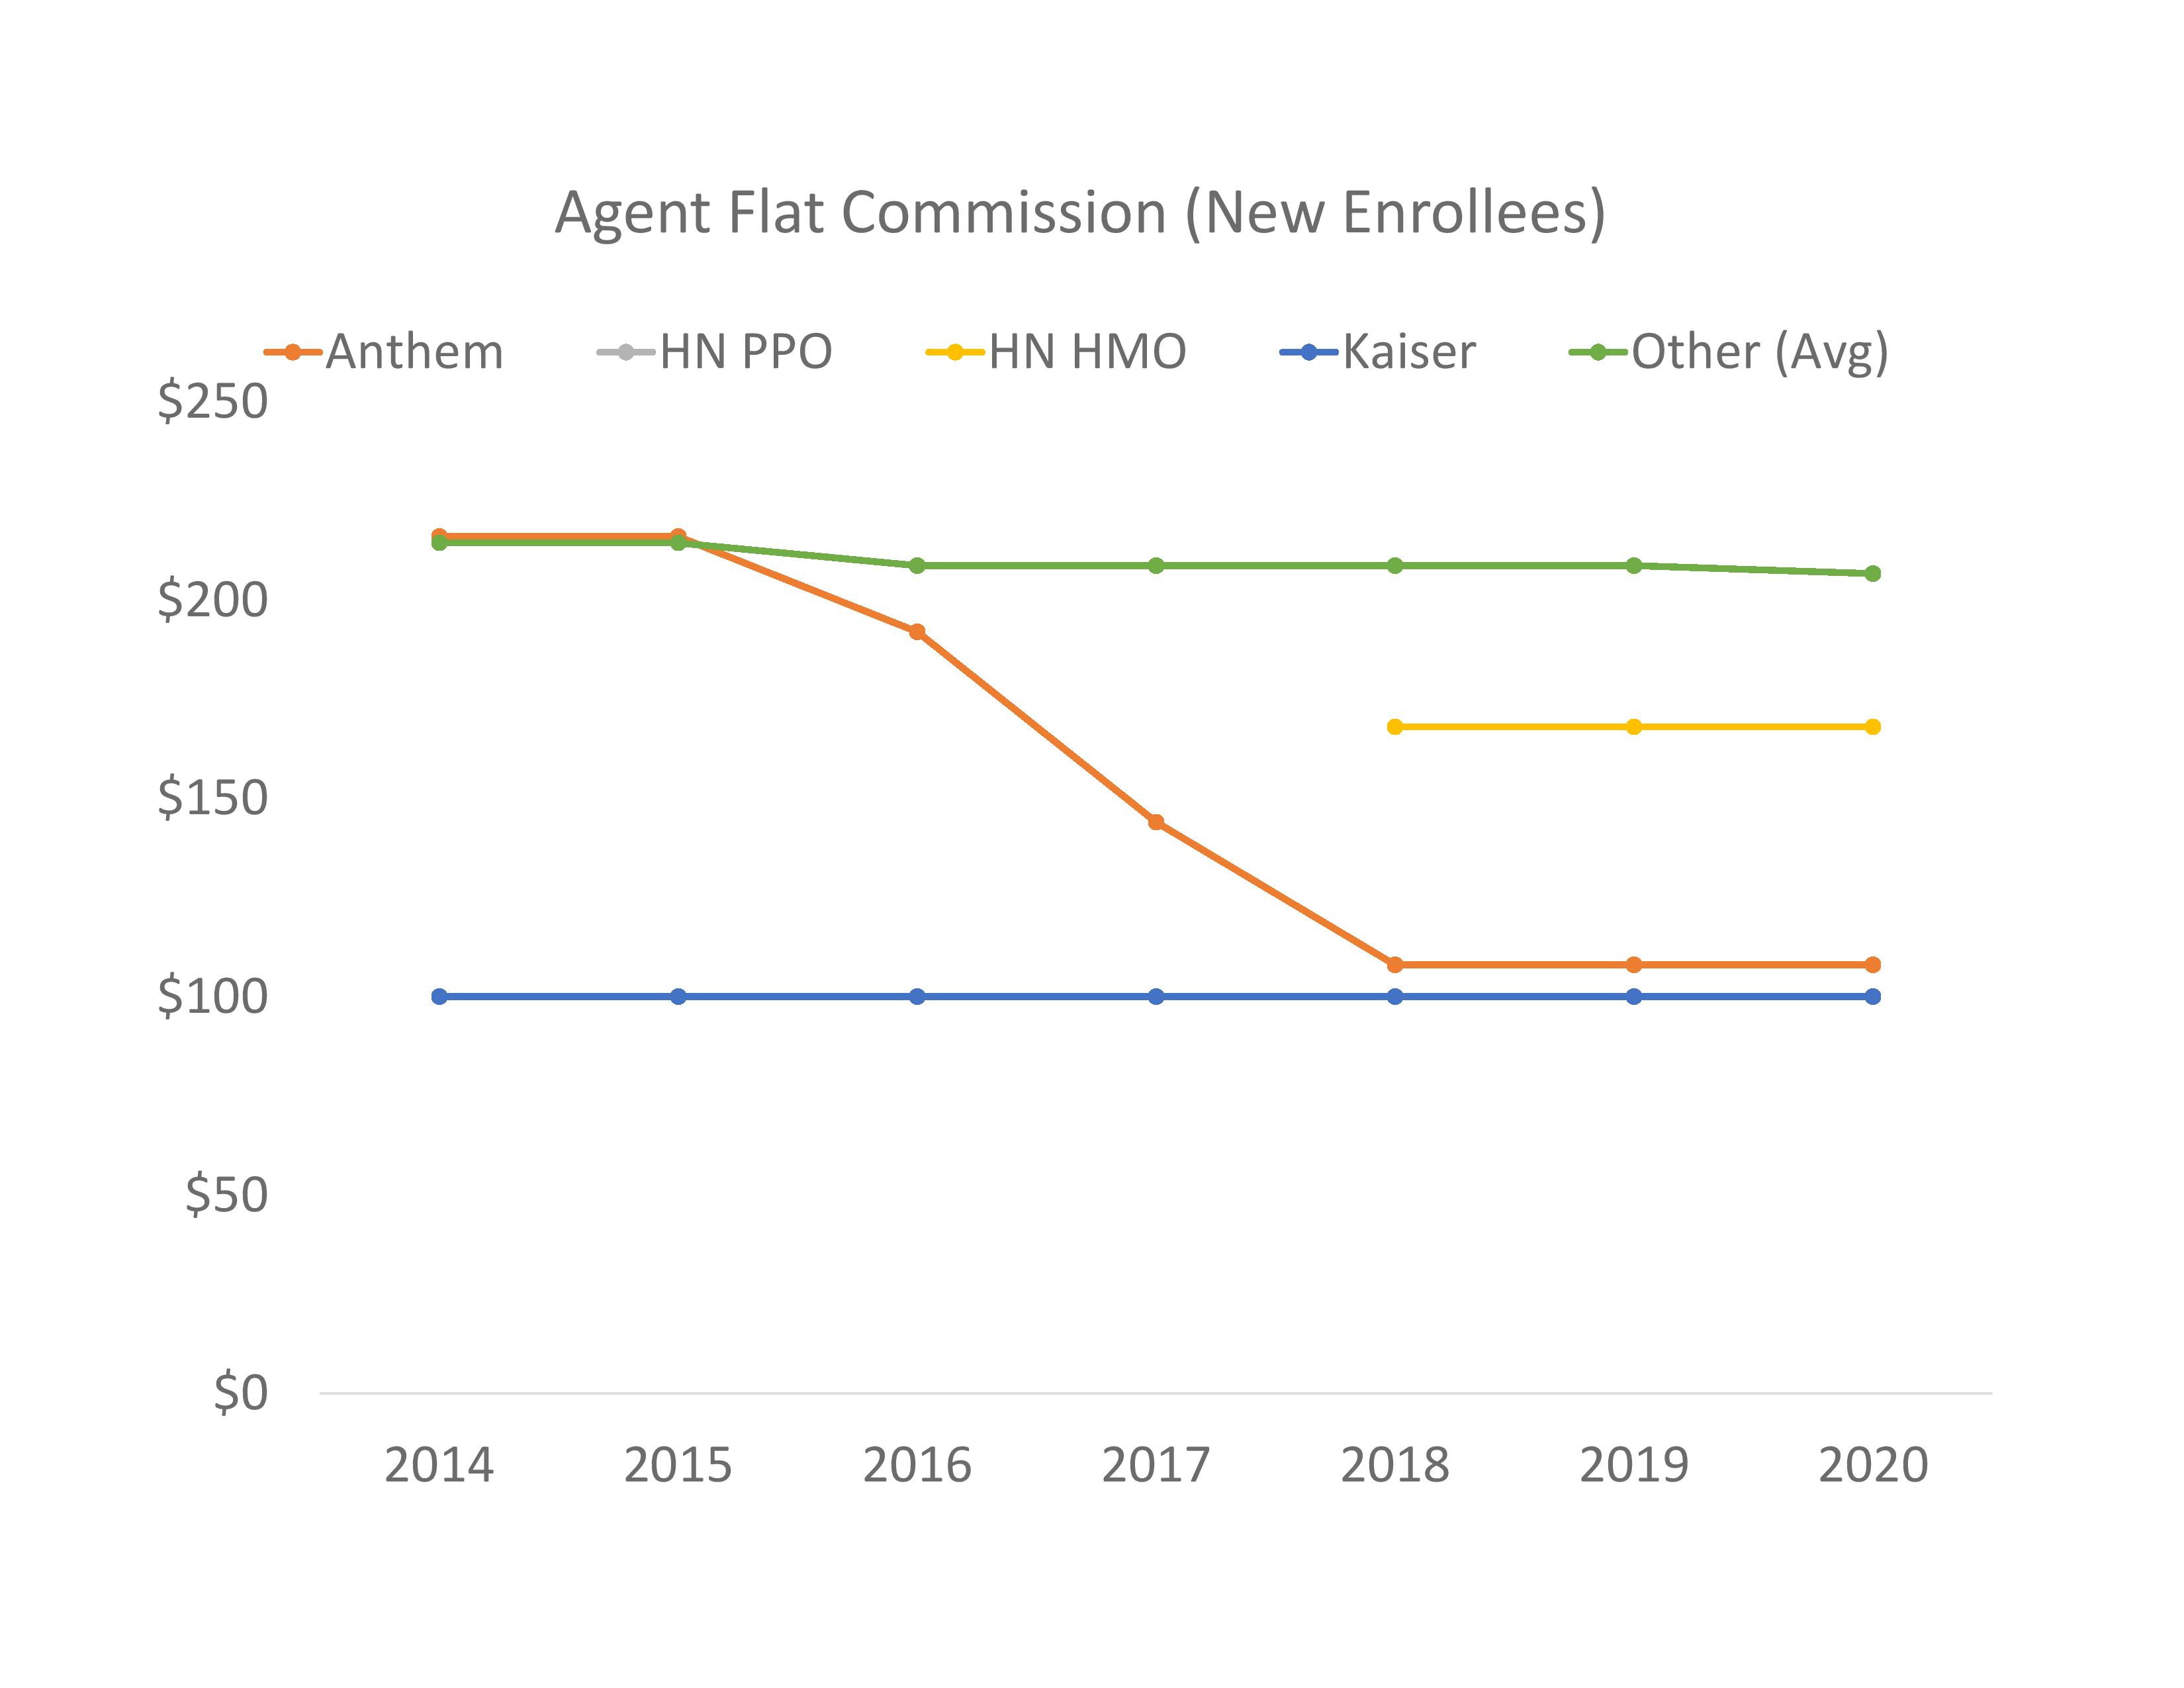
\includegraphics[scale=0.5]{finals/pics/flat_comm.jpg} \\
        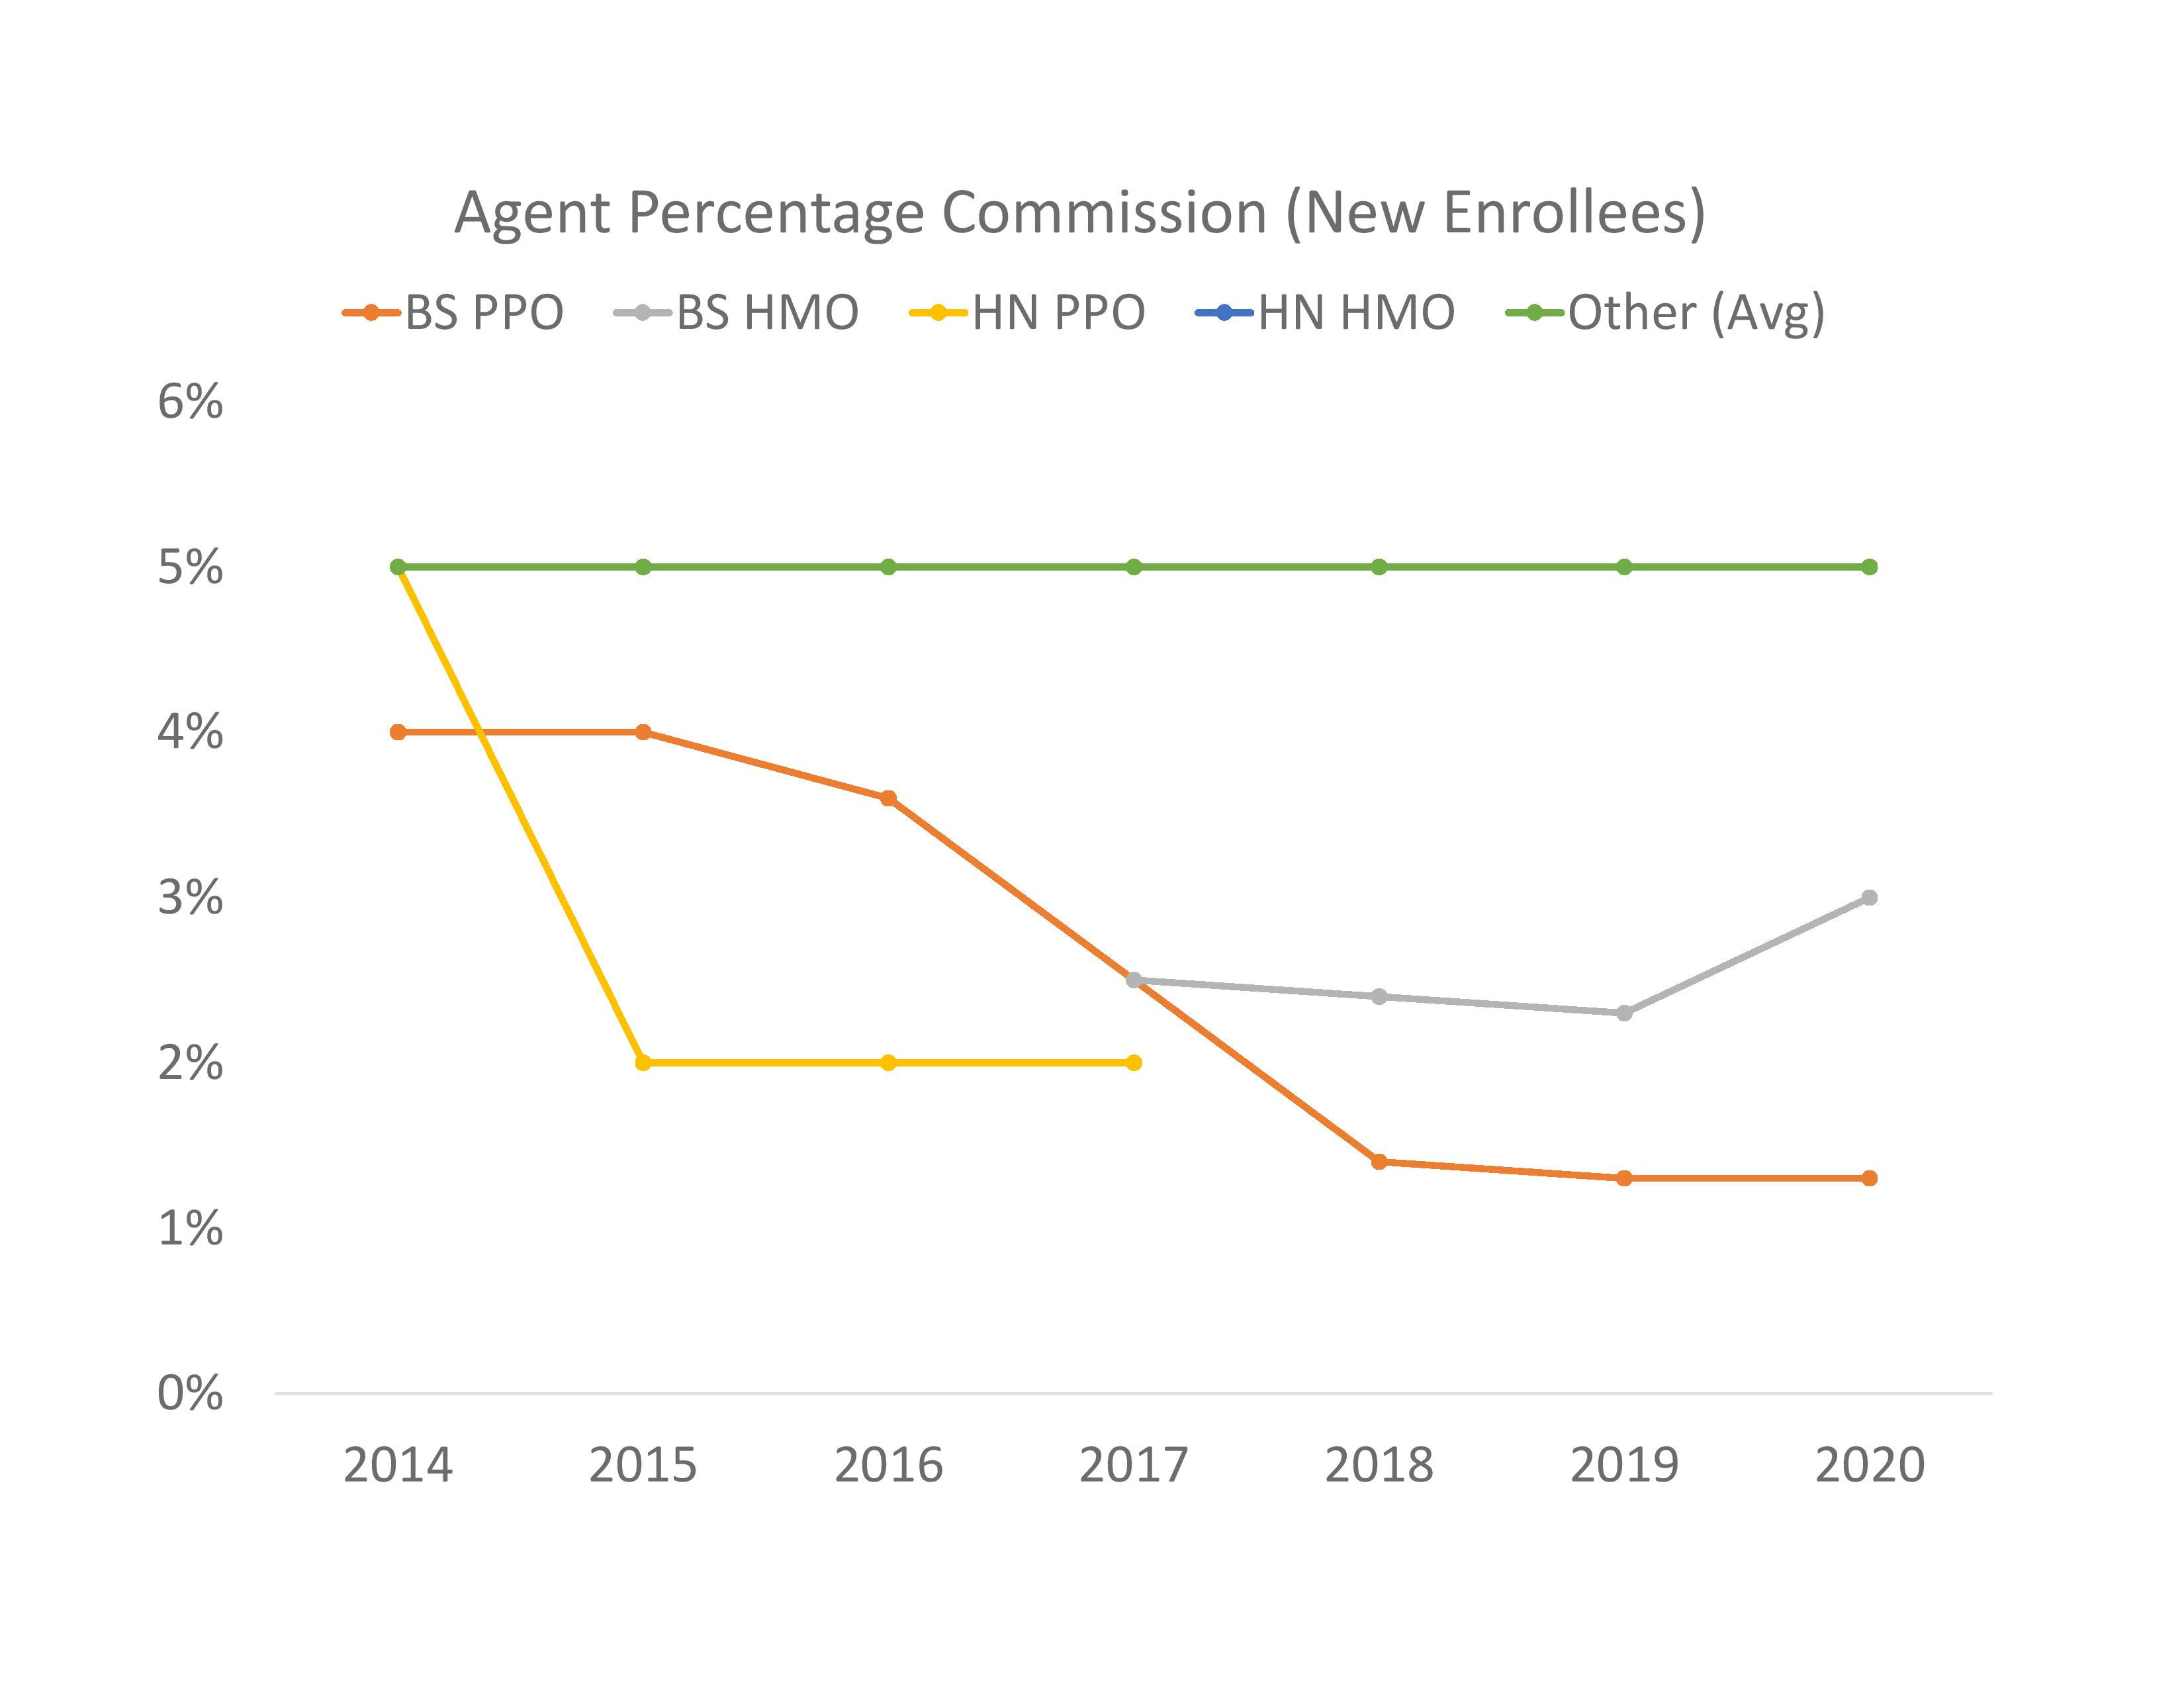
\includegraphics[scale=0.5]{finals/pics/perc_comm.jpg}
    \end{tabular}
}
\label{fig:commissions}
\end{minipage}
\end{figure}



\newpage
\begin{figure}[htb]
\caption{\textbf{Count of Enrollees in California Exchange}}
\centering
\begin{minipage}[h]{6in}
\centerline{%
    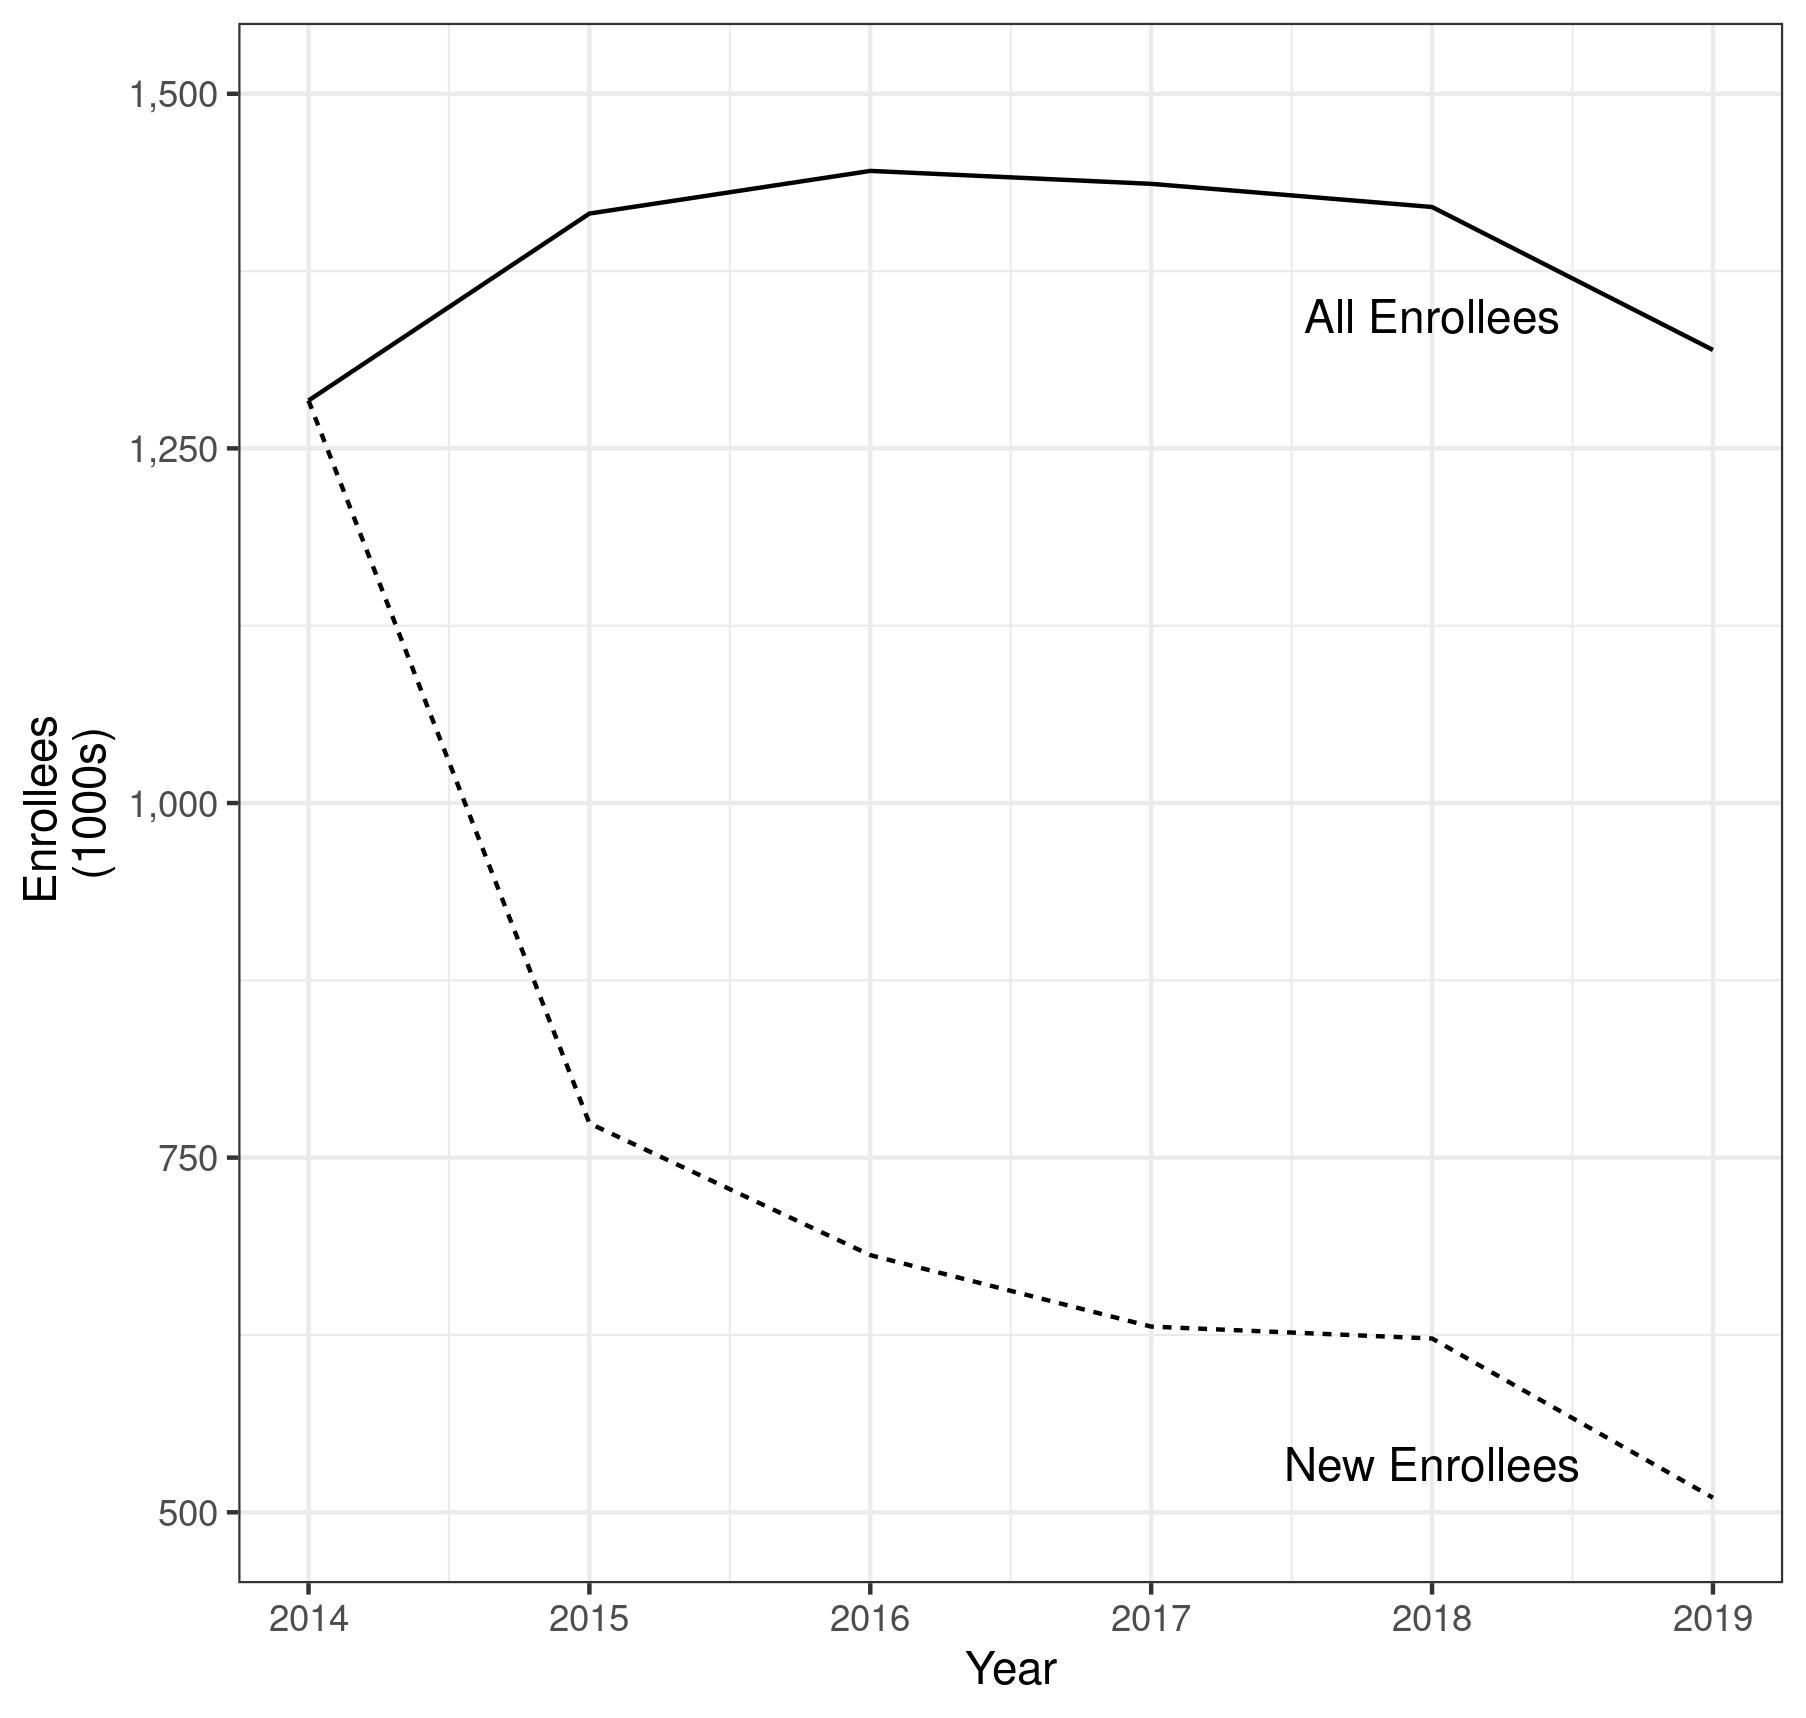
\includegraphics[scale=0.75]{figures/enrollee_count.png}
}
\label{fig:enrollee-count}
\end{minipage}
\end{figure}


\newpage
\begin{figure}[htb]
\centering
\footnotesize
\begin{minipage}[h]{6in}
\caption[caption]{\textbf{Histogram of Propensity Scores}\footnote{Propensity scores derived from a logistic regression of decision assistance on household characteristics, including the racial and ethnic makeup of the household, age of household members, gender of household members, household size, and household income. Regression analysis is limited to newly enrolled households, although results are comparable when considering all exchange households.}}
\centerline{%
    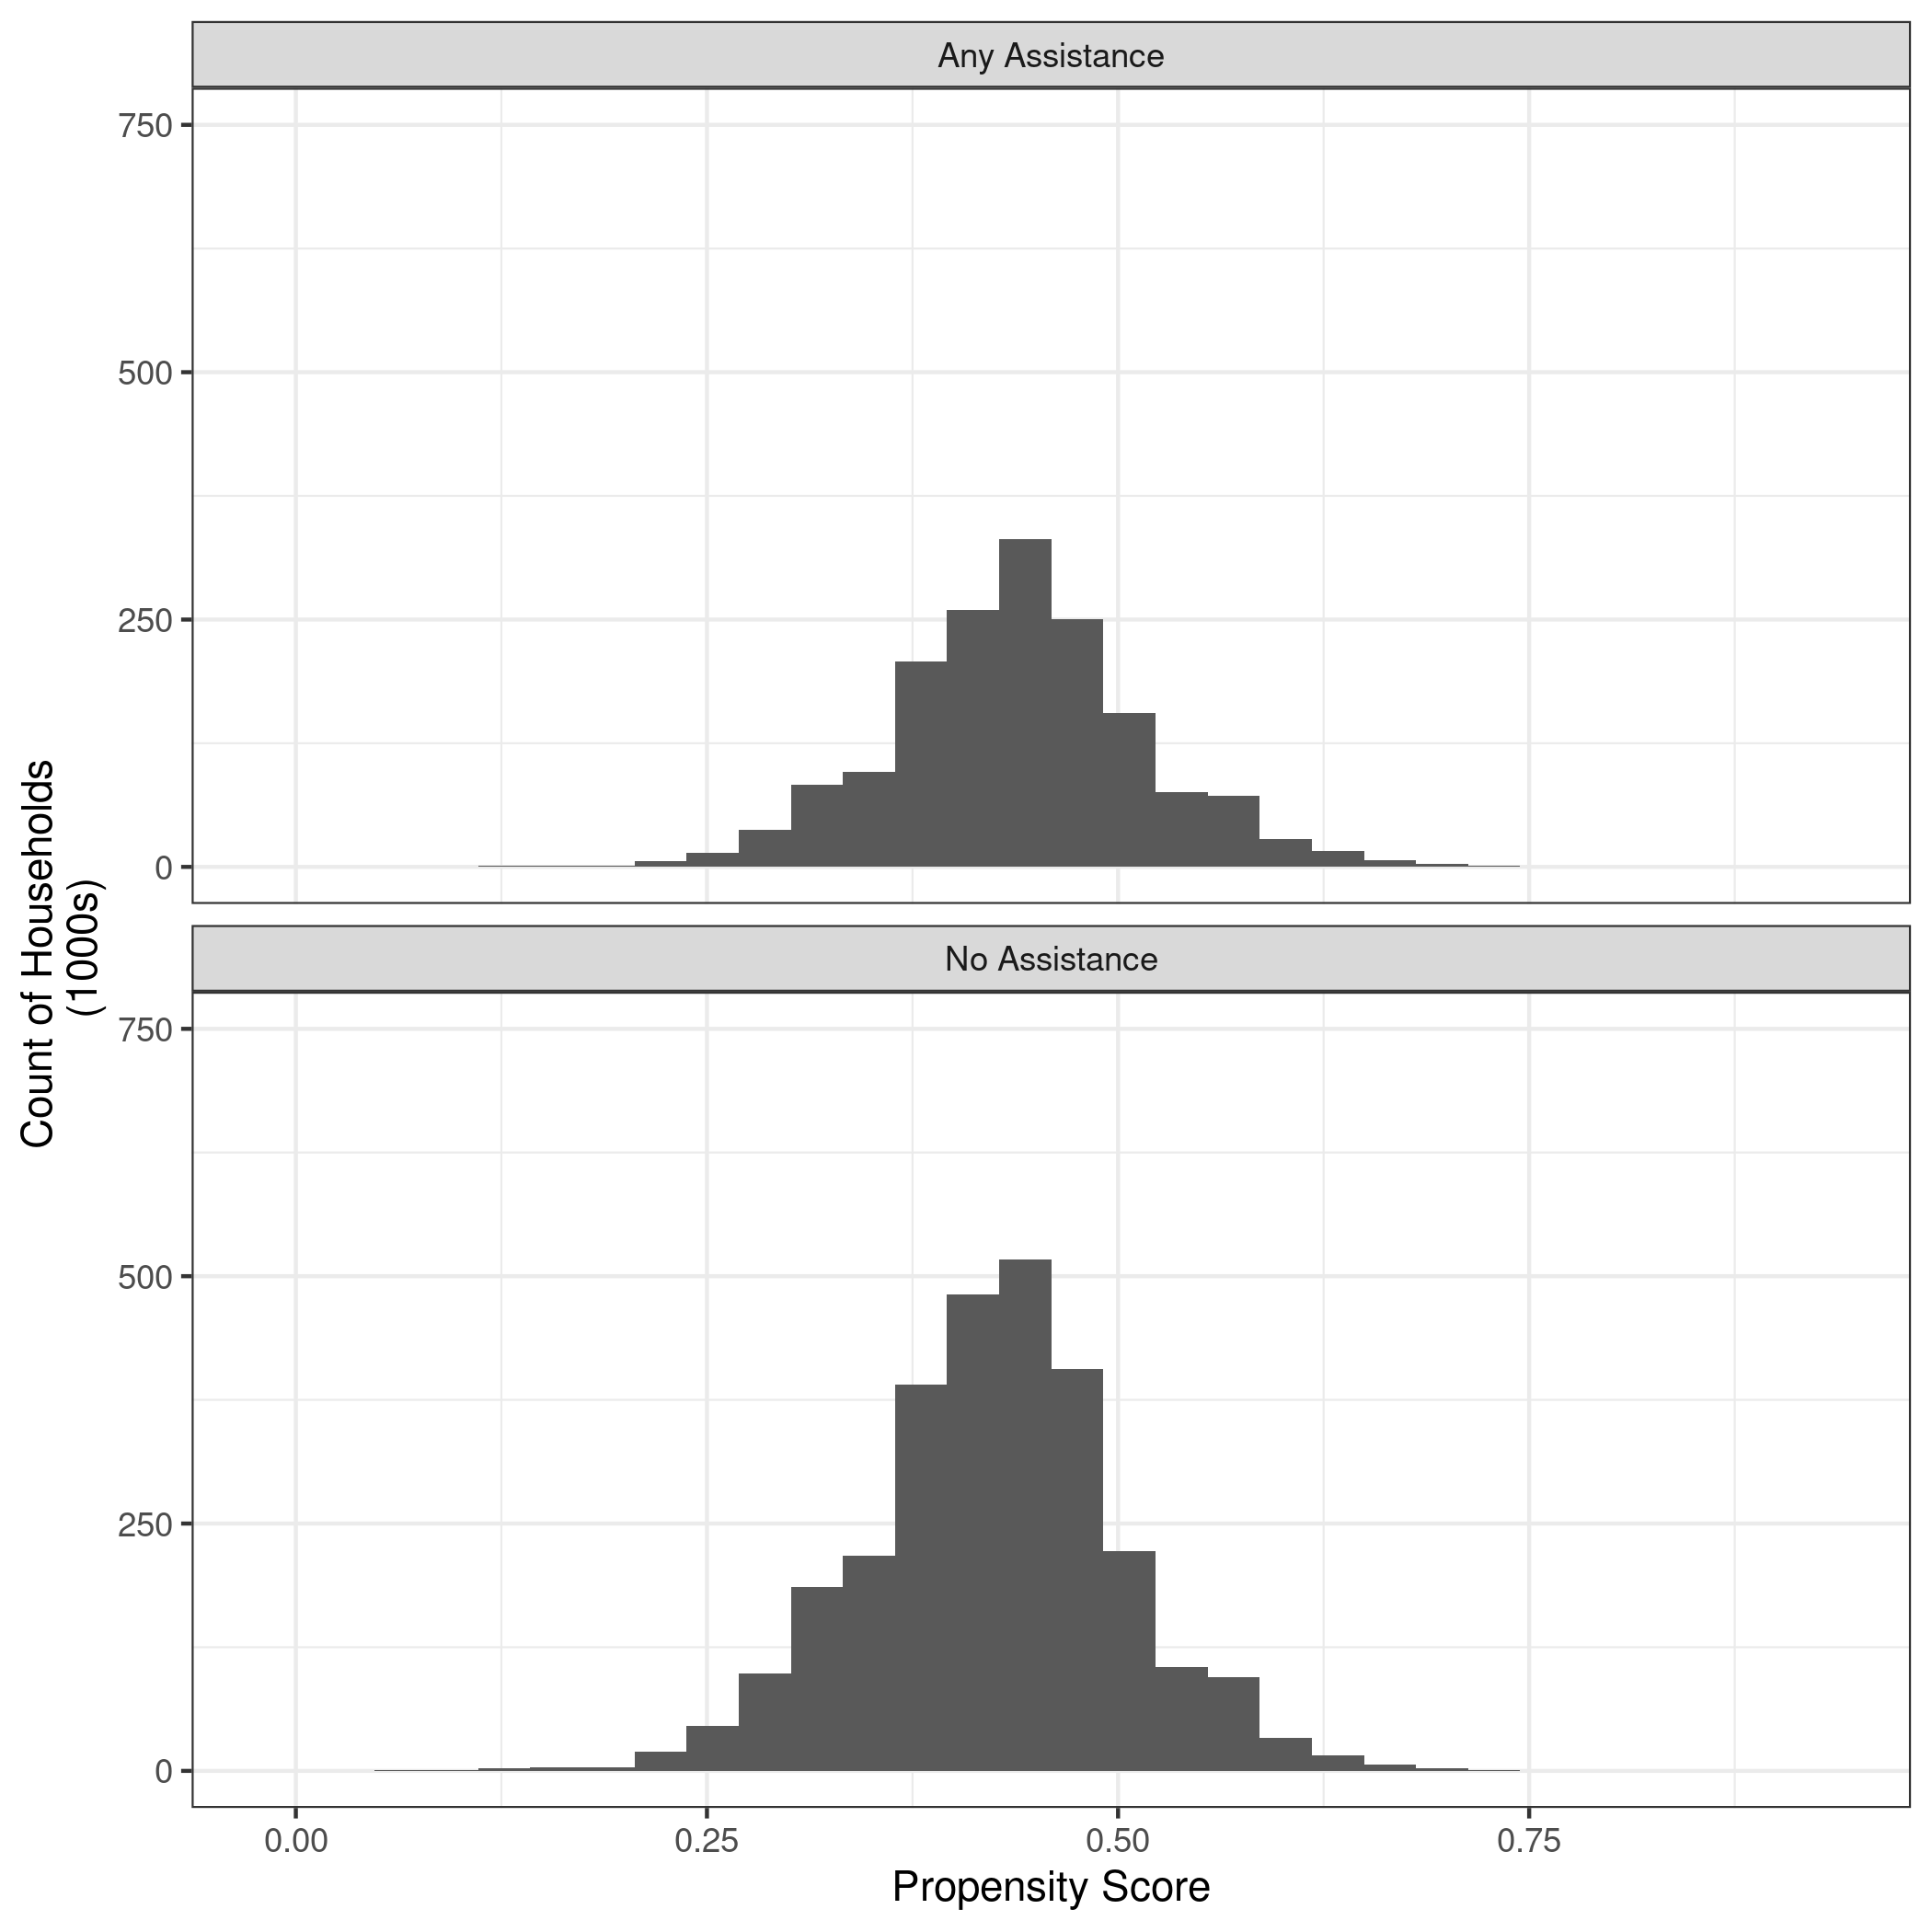
\includegraphics[scale=0.75]{figures/ps_assist_clean.png}
}
\label{fig:ps-balance}
\end{minipage}
\end{figure}


\newpage
\begin{figure}[htb]
\centering
\footnotesize
\begin{minipage}[h]{6in}
\caption[caption]{\textbf{Covariate Balance}\footnote{Standardized mean differences with and without inverse-propensity weighting, limited to newly enrolled households. ``IPW-ATT'' reflects weighted mean differences where treated households receive a weight of 1 and untreated households receive a weight of $p/(1-p)$ and where $p$ denotes the estimated propensity score from a logistic regression of decision assistance on observable household demographics (see Figure~\ref{fig:ps-balance}).}}
\centerline{%
    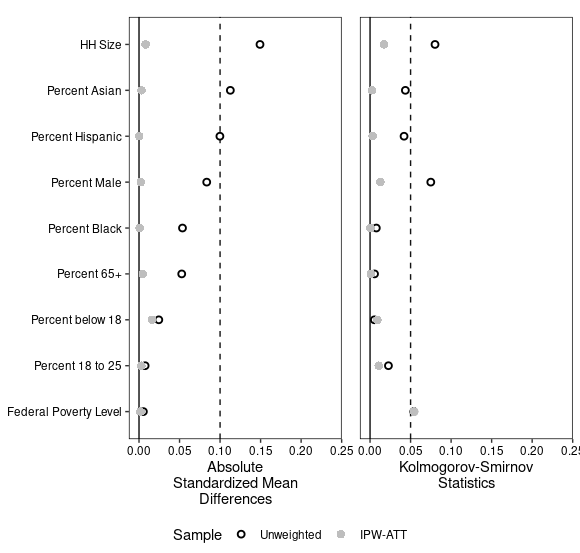
\includegraphics[scale=0.75]{figures/cov_balance.png}
}
\label{fig:cov-balance}
\end{minipage}
\end{figure}


\newpage
\begin{figure}[htb]
\centering
\footnotesize
\begin{minipage}[h]{6in}
\caption[caption]{\textbf{ATT of Decision Assistance on Insurer}\footnote{Estimated ATT as described in Section~\ref{sec:causal} aggregated to the insurer level. Confidence intervals derived from a paired bootstrap with 200 iterations.}}
\centerline{%
    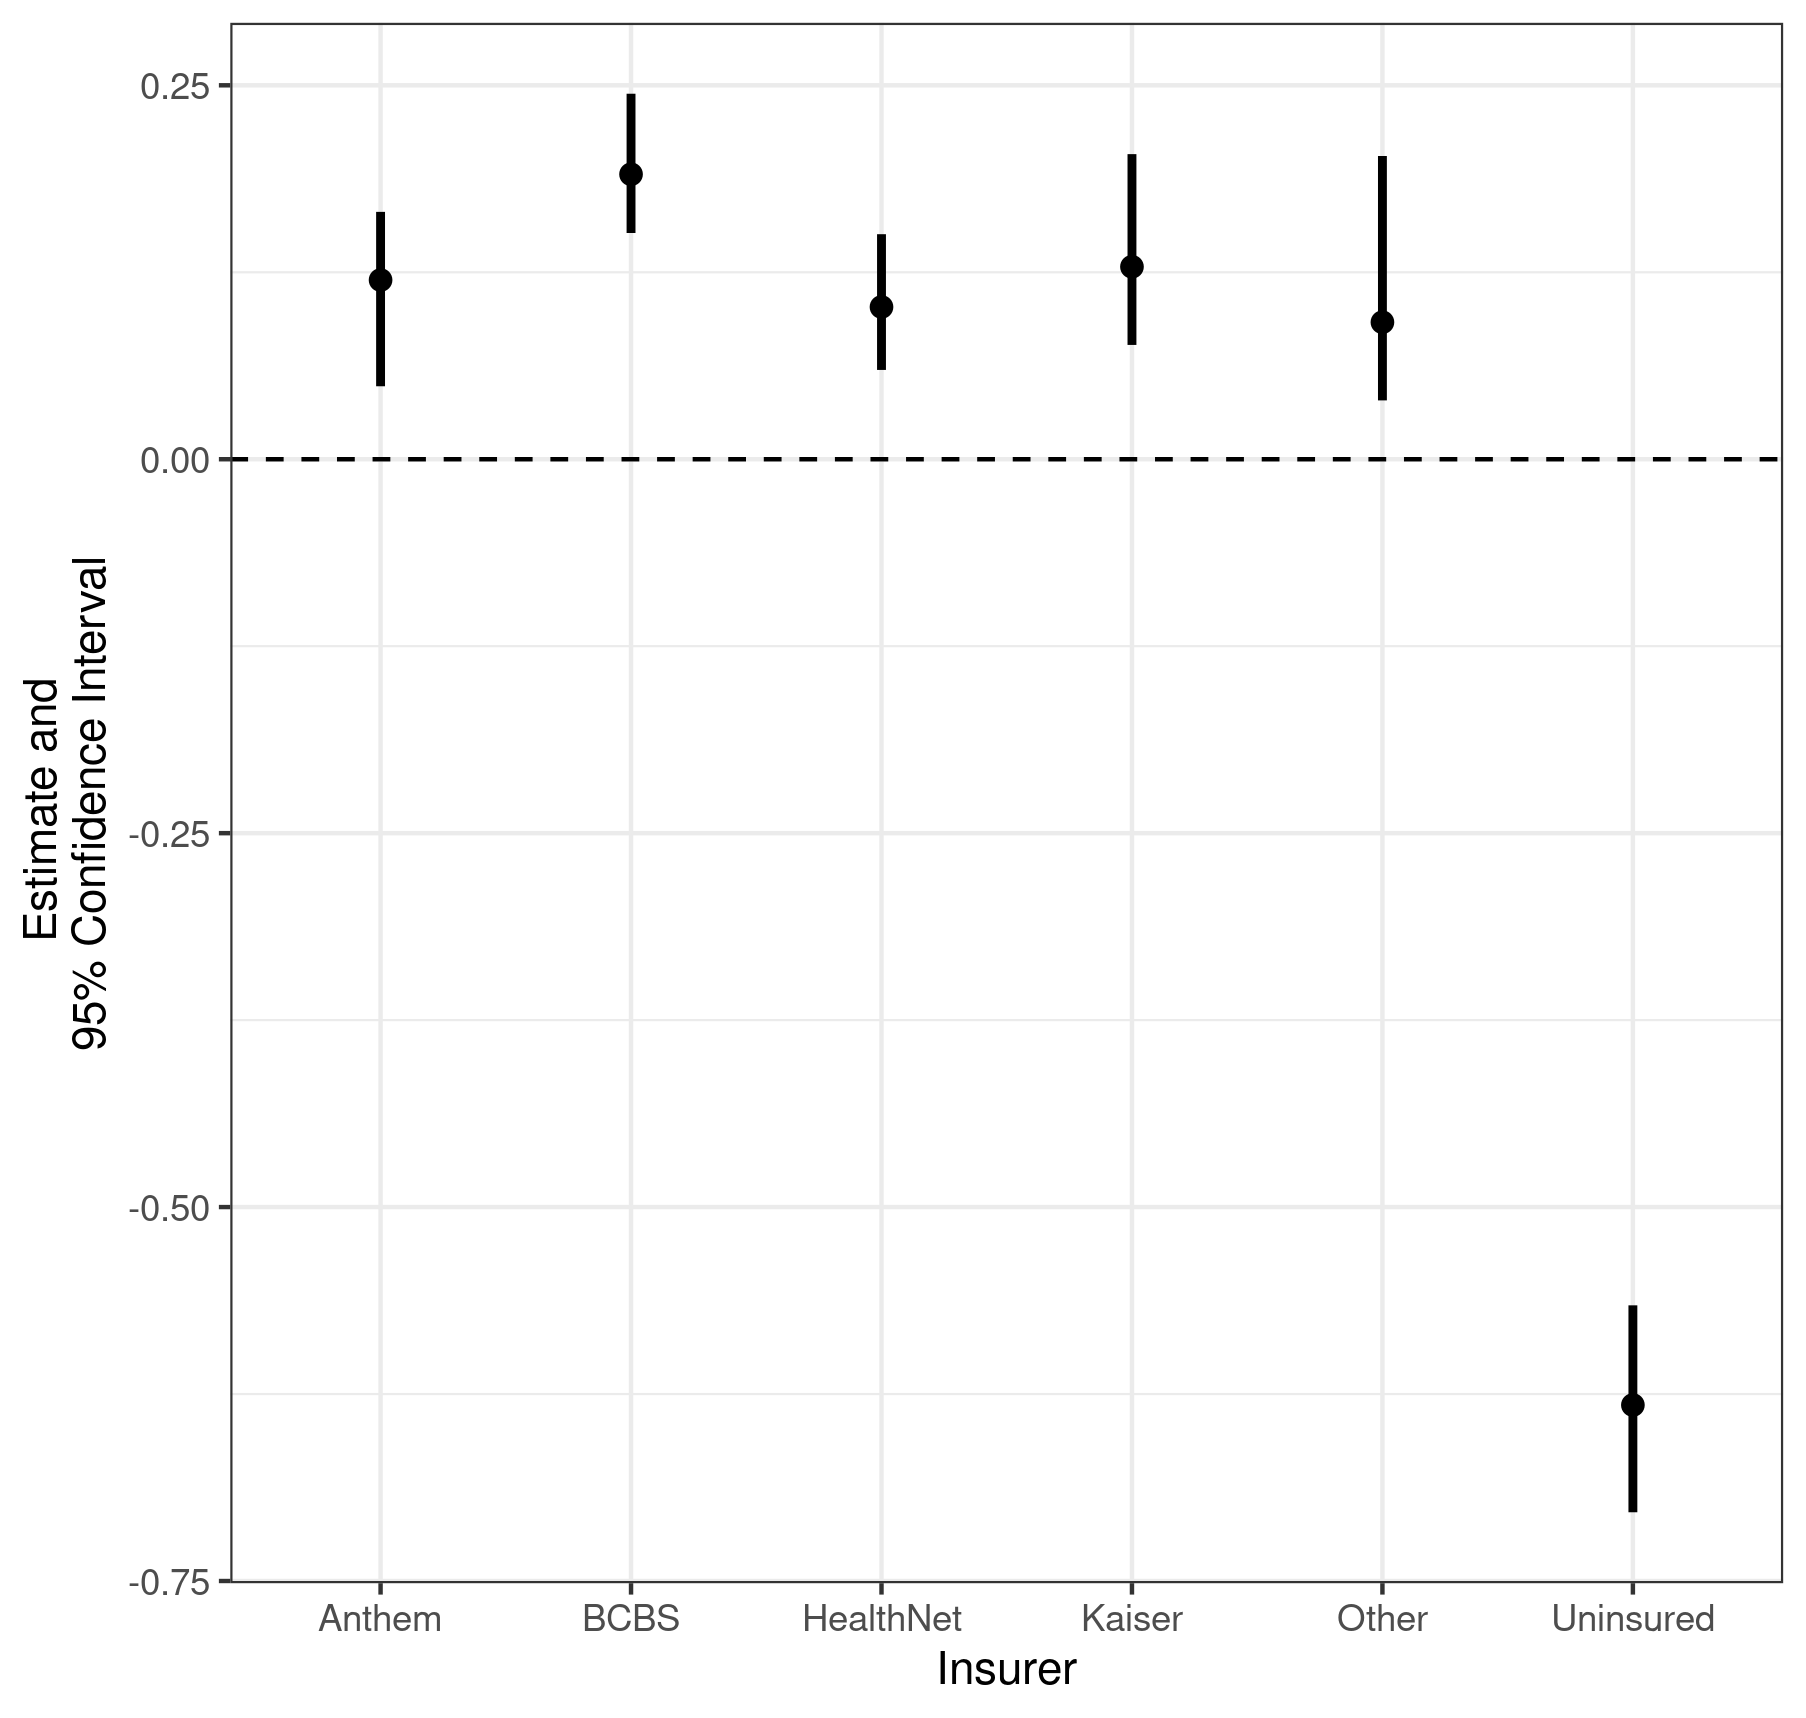
\includegraphics[scale=0.75]{figures/choice_insurer.png}
}
\label{fig:choice-insurer}
\end{minipage}
\end{figure}



\newpage
\begin{figure}[htb]
\centering
\footnotesize
\begin{minipage}[h]{6in}
\caption[caption]{\textbf{ATT of Decision Assistance on Metal Tier}\footnote{Estimated ATT as described in Section~\ref{sec:causal} aggregated to the level of metal tier. Confidence intervals derived from a paired bootstrap with 200 iterations.}}
\centerline{%
    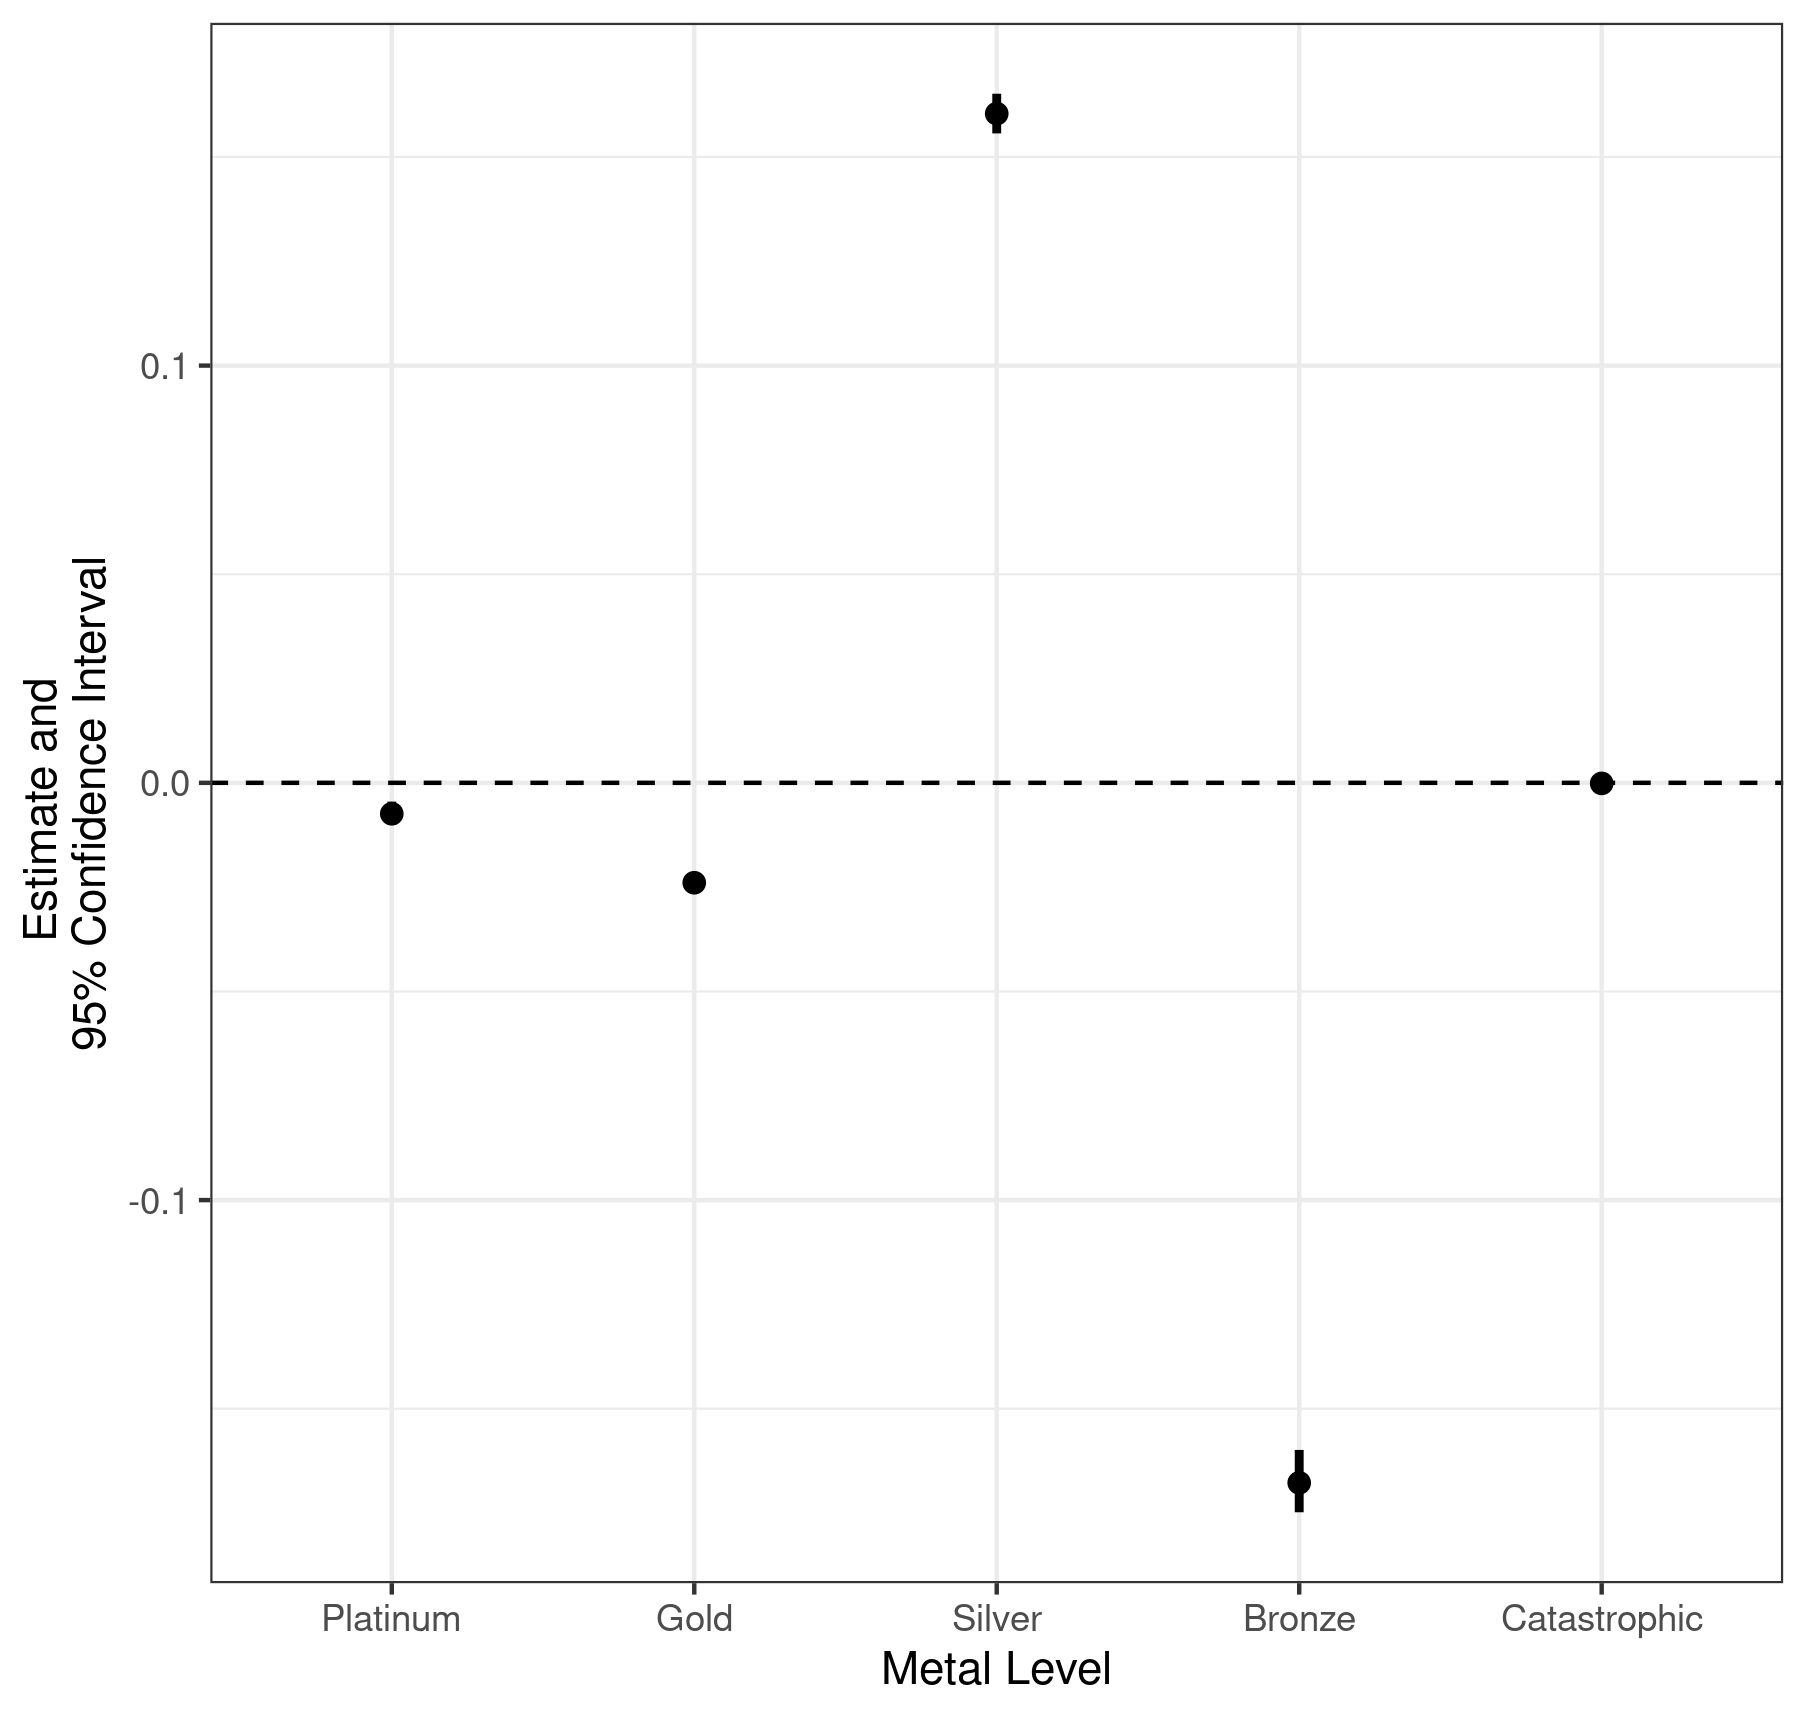
\includegraphics[scale=0.75]{figures/choice_metals.png}
}
\label{fig:choice-metal}
\end{minipage}
\end{figure}


\newpage
\begin{figure}[htb]
\centering
\footnotesize
\begin{minipage}[h]{6in}
\caption[caption]{\textbf{ATT of Decision Assistance on Dominated Choices}\footnote{Estimated ATT as described in Section~\ref{sec:dominated}. Confidence intervals derived from a paired bootstrap with 200 iterations.}}
\centerline{%
    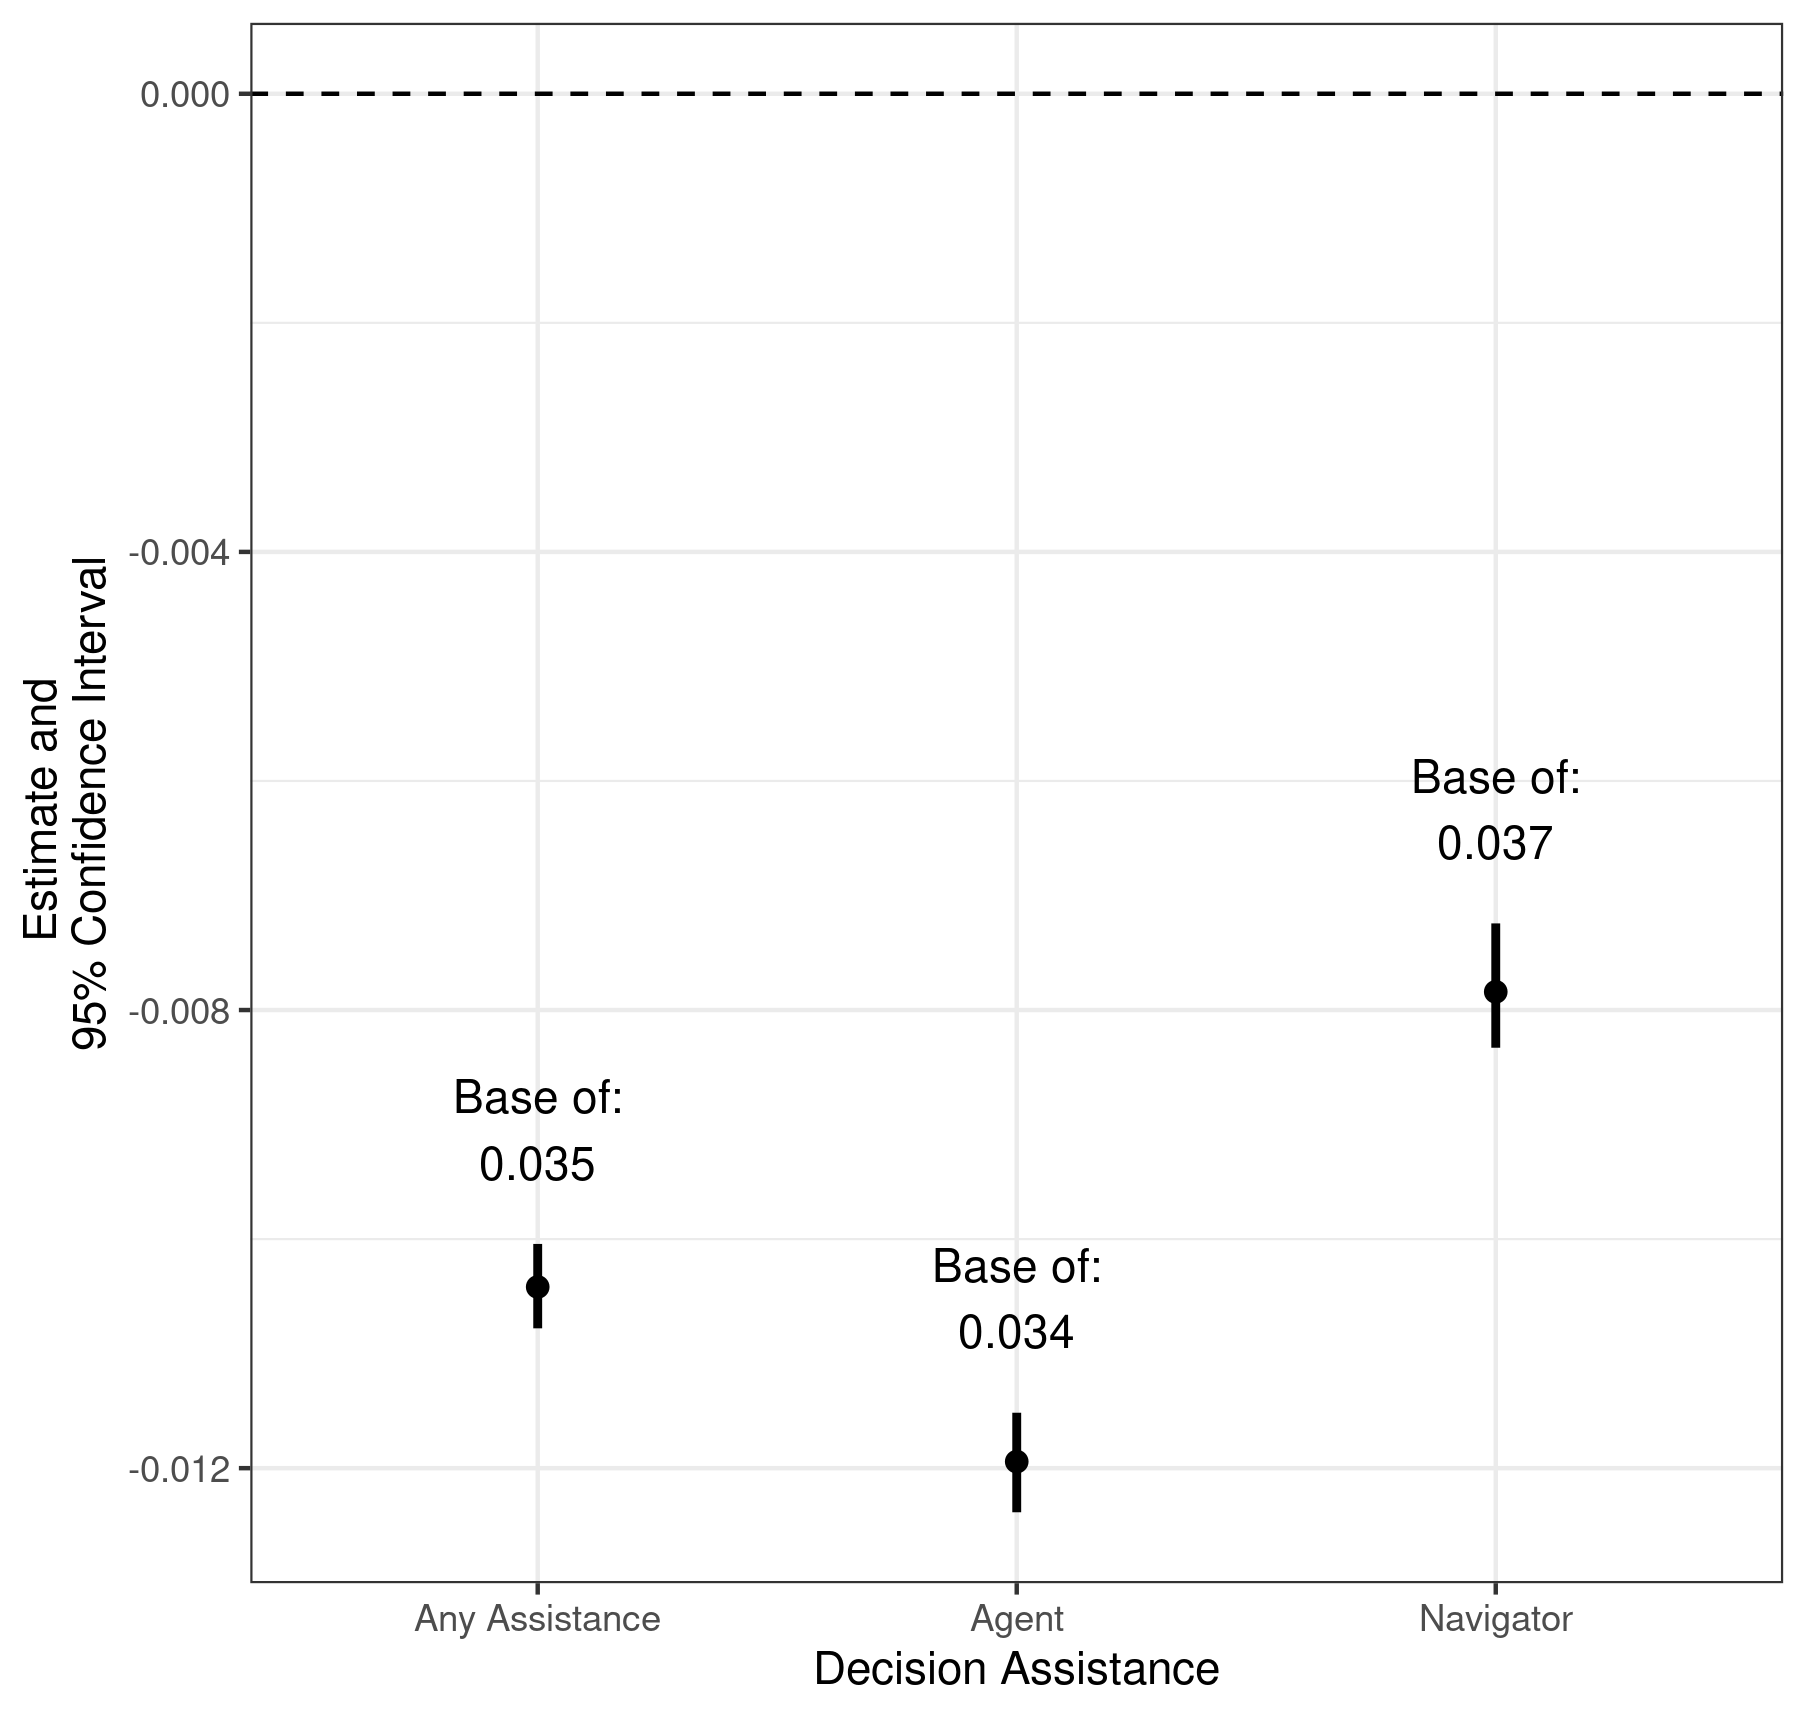
\includegraphics[scale=0.75]{figures/dom_choice.png}
}
\label{fig:dom-choice}
\end{minipage}
\end{figure}


\clearpage
\newpage
\begin{figure}[htb]
\centering
\footnotesize
\begin{minipage}[h]{6in}
\caption[caption]{\textbf{Premium Rating Regions in California}\footnote{Premium rating regions in the California exchange \citep{CARATE2016}. California's 58 counties are divided into 19 rating areas.}}
\centerline{%
    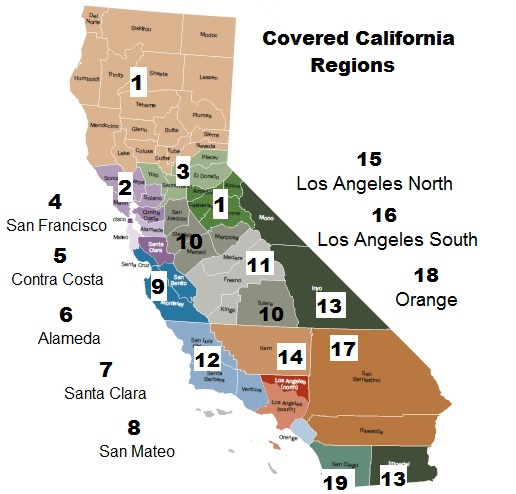
\includegraphics[scale=.45]{finals/pics/CA_Rating_Regions2.jpg}	
}
\label{rating_area_partitions}
\end{minipage}
\end{figure}  



\end{document}


